% GENERATED FROM typst/sections/06_field.typ BY scripts/typ2tex.py (v1.0.0) — DO NOT EDIT.
% Edit canonical Typst under typst/ and regenerate with: python3 scripts/typ2tex.py --root . --outdir latex

\section{Field and SADAR}\label{sec:stokes-sadar-harmonic}
\label{sec:afc-stokes-seed}
\label{subsec:afc-stokes-identity}

The finite flux and response constructions retain their declared channel histories.
For a committed value trace of \eqref{eq:wave-identity}, the harmonic
representation begins at \eqref{eq:fourier-transform}.

\subsection{Typed finite flux}

\paragraph{Setup.}
AFC declares normalized memory $p_i^{\mathrm{mem}}\ge0$, $\sum_ip_i^{\mathrm{mem}}=1$,
and a stochastic kernel $P$. A$\Omega$D separately resolves pressure-bearing
values of admitted returned channels. Keep their types explicit:

\begin{equation}\label{eq:flux-types}
\varphi^{\mathrm{AFC}}_{ij}=p_i^{\mathrm{mem}}P_{ij}-p_j^{\mathrm{mem}}P_{ji},\qquad\varphi^{\mathrm{AOD}}_{ij}(B)=p^D_{ij}(B)A_{ij}(B).
\end{equation}

Each normalized product lies in $[0,1]$, hence
$|\varphi^{\mathrm{AFC}}_{ij}|\le1$. A$\Omega$D pressure-bearing channel values
use their declared count domain. Orientation reversal of a
fixed antisymmetric flux changes its sign. A separately constructed reverse
channel retains its own directional RCD and need not have the same magnitude.

\paragraph{Joint invariance.}
For a relabelling $g$, $p^{\mathrm{mem}}_{gi}=p^{\mathrm{mem}}_i$ and
$P_{gi,gj}=P_{ij}$ imply $\varphi^{\mathrm{AFC}}_{gi,gj}=\varphi^{\mathrm{AFC}}_{ij}$
by substitution. With only kernel invariance, the flux difference is

\[
\varphi^{\mathrm{AFC}}_{gi,gj}-\varphi^{\mathrm{AFC}}_{ij}=(p^{\mathrm{mem}}_{gi}-p^{\mathrm{mem}}_i)P_{ij}-(p^{\mathrm{mem}}_{gj}-p^{\mathrm{mem}}_j)P_{ji},
\]

which need not vanish.

\paragraph{Region and boundary.}
Let $V$ be the finite vertex set, $R\subseteq V$, and
$\partial R=\{(i,j):i\in R,j\notin R\}$ its oriented cut.

\begin{equation}\label{eq:b-scoped-divergence}
\operatorname{div}(i;B)=\sum_{j\in V}\varphi_{ij}(B).
\end{equation}

\subsubsection{Finite Stokes}

\paragraph{Derivation.}
For either one declared antisymmetric flux type, split the double sum:

\begin{equation}\label{eq:afc-stokes-used}
\begin{aligned}
\sum_{i\in R}\operatorname{div}(i;B) & =\sum_{i,j\in R}\varphi_{ij}(B)+\sum_{i\in R,j\notin R}\varphi_{ij}(B)\\ & =\sum_{i\in R,j\notin R}\varphi_{ij}(B).
\end{aligned}
\end{equation}

The internal sum is zero because each ordered pair cancels its reverse and
diagonal entries are zero. Cancellation removes a summed value, not the
two contributing lineage records. The same finite argument holds componentwise.

\begin{equation}\label{eq:afc-flux-ao-resolution}
\varphi^{\mathrm{AOD}}_{ij,\AO}(B)=p^D_{ij,\AO}(B)A_{ij,\AO}(B).
\end{equation}

In the remaining pressure formulas $\varphi$ abbreviates $\varphi^{\mathrm{AOD}}$.

\paragraph{Falsification.}Wrong antisymmetry or an omitted boundary channel
breaks the finite identity.

\aodprovenance{\eqref{eq:rcd-coupling},
\eqref{eq:flux-types},
\eqref{eq:afc-stokes-used}.}

\aodliteraturenote{AFC Choices (memory, stochastic kernel, flux) and
Stokes corollary, finite internal-pair cancellation: Poyau~\cite{afc},
Choices~1--5, Corollary~1 and equation~(1),
source revision \href{https://github.com/rpoyau/afc/commit/5a25e8bd5bbc3f20ec4413a6b63abc420b7a54cb}{\texttt{5a25e8bd5bbc}}.}

\subsubsection{$B$-scoped flux contents}\label{subsec:b-scoped-flux-contents}

Resolve the A$\Omega$D channel operands of \eqref{eq:flux-types} on
$B=(\partial F,\omega)$.

For a declared path-history family $\mathcal{H}_{ij}(B)$, the path-history pressure is

\begin{equation}\label{eq:path-history-pressure}
p^D_{ij}(B)=\sum_{h\in\mathcal{H}_{ij}(B)}C_{3,h}\rho^D_{\omega,h}(B).
\end{equation}

A compressed channel form is licensed only after the declared compression

\begin{equation}\label{eq:path-history-compression}
\mathsf{Comp}_{ij}:\{(C_{3,h},RD_h,R^{\mathrm{asym}}_h,A_h)\}_{h\in\mathcal{H}_{ij}(B)}\mapsto(C_{3,ij},\rho^D_{ij},A_{ij}).
\end{equation}

Under that declared compression,

\begin{equation}\label{eq:b-scoped-channel-pressure}
p^D_{ij}(B)=C_{3,ij}\rho^D_{\omega,ij}(B)=C_{3,ij}\min(\rho^D_{ij}(B),|\omega|_{ij}).
\end{equation}

The bare-duration form is the neutral-reflection reduction:

\[
R^{\mathrm{asym}}_{ij}(B)=\mathrm{id}\quad\Rightarrow\quad\rho^D_{ij}(B)=D_{ij}(B).
\]

The direction term is

\begin{equation}\label{eq:b-scoped-channel-attention}
A_{ij}(B)=\Delta\chi^{\mathrm{lag}}_{ij}(B)i_{ij}(B).
\end{equation}

The A$\Omega$D branch of \eqref{eq:flux-types} gives

\begin{equation}\label{eq:b-scoped-flux}
\varphi_{ij}(B)=p^D_{ij}(B)A_{ij}(B).
\end{equation}

Equivalently,

\begin{equation}\label{eq:b-scoped-flux-expanded}
\varphi_{ij}(B)=C_{3,ij}\rho^D_{\omega,ij}(B)\Delta\chi^{\mathrm{lag}}_{ij}(B)i_{ij}(B).
\end{equation}

\paragraph{Magnitude and direction.}
In \eqref{eq:b-scoped-flux}, $p^D$ is magnitude and $A$ is direction.
Scaling every $p^D$ by $\lambda$ at fixed orientation and channel family
scales both $\varphi$ and its attention sum $\mathbf{A}_F$ by $\lambda$.

For a fixed antisymmetric flux on the oriented pair $(i,j)$:

\begin{equation}\label{eq:b-scoped-flux-antisymmetry}
\varphi_{ji}(B)=-\varphi_{ij}(B),\qquad\varphi_{ii}(B)=0.
\end{equation}

When $i_{ij}(B)$ has components, the antisymmetry and Stokes identity are evaluated componentwise.

The divergence is the sum defined in \eqref{eq:b-scoped-divergence}.

Specializing \eqref{eq:afc-stokes-used} to this flux gives

\begin{equation}\label{eq:b-scoped-stokes}
\sum_{i\in R}\operatorname{div}(i;B)=\sum_{\substack{i\in R\\j\notin R}}\varphi_{ij}(B).
\end{equation}

\begin{figure}[H]
\centering
\fbox{\begin{minipage}{0.94\linewidth}\centering
\textbf{SADAR as $B$-scoped A$\Omega$D flux} 

{\footnotesize
\begin{tabularx}{\linewidth}{>{\raggedright\arraybackslash}p{0.280\linewidth}>{\raggedright\arraybackslash}p{0.050\linewidth}>{\raggedright\arraybackslash}X}
Scope & $\to$ & $B=(\partial F,\omega)$ \\
RCD & $\to$ & $\operatorname{RCD}_{ij}(B)=RD_B(C_{ij})\bowtie_BR^{\mathrm{asym}}_{ij}(B)$ \\
Scalar duration & $\to$ & $\rho^D_{ij}(B)=\operatorname{dur}(\operatorname{RCD}_{ij}(B))$ \\
Window clip & $\to$ & $\rho^D_{\omega,ij}(B)=\min(\rho^D_{ij}(B),|\omega|_{ij})$ \\
Magnitude & $\to$ & $p^D_{ij}(B)=C_{3,ij}\rho^D_{\omega,ij}(B)$ \\
Direction & $\to$ & $A_{ij}(B)=\Delta\chi^{\mathrm{lag}}_{ij}(B)i_{ij}(B)$ \\
Flux & $\to$ & $\varphi_{ij}(B)=p^D_{ij}(B)A_{ij}(B)$ \\
Attention & $\to$ & $\mathbf{A}_F(B)=\sum_{(i,j)\in F(B)}\varphi_{ij}(B)$ \\
Motion & $\to$ & $(S^W_k,S^W_{k+1})\text{ under }\mathcal{U}_B$ \\
\end{tabularx}
}
\end{minipage}}
\caption{SADAR as $B$-scoped A$\Omega$D flux.}
\label{fig:sadar-b-scoped-afc-flux}
\end{figure}

\aodprovenance{\eqnref{eq:afc-stokes-used}; \eqnref{eq:afc-flux-ao-resolution}; \eqnref{eq:b-scoped-flux}; \eqnref{eq:b-scoped-stokes}.}

\subsubsection{Slice flux}\label{subsec:slice-flux}

\begin{definition}[Duon slice flux]
For a declared cut-frame $t$, let

\[
B|_t=(\partial F,\{t\}).
\]

The duon-current slice flux is the one cut-frame crossing

\begin{equation}\label{eq:slice-flux}
\Phi^D_{\partial R}(t;B|_t)=\sum_{e\in\partial R(t)}\varphi_e(B|_t).
\end{equation}

When the scope is fixed, write $\Phi^D_{\partial R}(t)$. For raw duon-current content, $\varphi_e(B|_t)=\epsilon_eC_{3,e}$.
\end{definition}

\subsubsection{Window current}\label{subsec:window-current}

\begin{definition}[Window duon current]
The window current is the retained many-frame continuation

\begin{equation}\label{eq:window-current}
J^D_{\partial R}(\omega;B)=\sum_{t\in\omega}\Phi^D_{\partial R}(t;B|_t).
\end{equation}

When the scope is fixed, write $J^D_{\partial R}(\omega)$.
\end{definition}

The raw capacity crossing count is

\begin{equation}\label{eq:raw-capacity-crossing-count}
N^D_{\partial R}(\omega;B)=\sum_{t\in\omega}\sum_{e\in\partial R(t)}C_{3,e}.
\end{equation}

The magnitude current is

\begin{equation}\label{eq:magnitude-current}
J^D_{\mathrm{mag}}(\omega;B)=\sum_{t\in\omega}\sum_{e\in\partial R(t)}p^D_e(B|_t).
\end{equation}

When the declared boundary/window partitions current status, require

\begin{equation}\label{eq:current-magnitude-split}
J^D_{\mathrm{mag}}=J^D_{\mathrm{in}}+J^D_{\mathrm{out}}+J^D_{\mathrm{pending}}.
\end{equation}

\subsubsection{Moving boundary}\label{subsec:moving-boundary}

For a moving retained boundary, the window may record crossing, sweep, and shedding terms as

\begin{equation}\label{eq:moving-boundary}
\Phi^D_{\partial R,\mathrm{mov}}(t)=\Phi^D_{\mathrm{cross}}(t)-\Phi^D_{\mathrm{sweep}}(t)+\Phi^D_{\mathrm{shedding}}(t).
\end{equation}

Here crossing is duon current crossing the retained boundary, sweep is support swept by boundary motion, and shedding is disturbance that breaks from the retained boundary.

\subsubsection{Regional boundary template}\label{subsec:regional-boundary-template}

The same boundary/current form applies across familiar region choices. Declare a region, declare $\partial R$, and account for current crossing, returning, and remaining pending.

\begin{figure}[H]
\centering
\fbox{\begin{minipage}{0.94\linewidth}\centering
\textbf{Duon-current boundary accounting} 

{\footnotesize
\begin{tabular}{>{\raggedright\arraybackslash}p{0.230\linewidth}>{\raggedright\arraybackslash}p{0.230\linewidth}>{\raggedright\arraybackslash}p{0.230\linewidth}>{\raggedright\arraybackslash}p{0.230\linewidth}}
\textbf{Internal retained} & \textbf{Exoshedding} & \textbf{Reflected return} & \textbf{Pending return} \\
recurring core & crosses $\partial R$ & returns through shell & remains over $\omega$ \\
scalar burden & shell crossing & next emission & duration overlap \\
\end{tabular}
}

$\Phi^D_{\partial R}(t;B|_t)=\sum_{e\in\partial R(t)}\varphi_e(B|_t)$ 

$J^D_{\partial R}(\omega;B)=\sum_{t\in\omega}\Phi^D_{\partial R}(t;B|_t)$
\end{minipage}}
\caption{Duon-current boundary accounting.}
\label{fig:v39-duon-current-boundary-accounting}
\end{figure}

\aodprovenance{\eqnref{eq:duon-current},
\eqnref{eq:slice-flux},
\eqnref{eq:window-current},
\eqnref{eq:moving-boundary}.}

\subsection{Field count}\label{sec:field-count-sadar-scope}

\subsubsection{Scope}\label{subsec:field-count-fixed-scope}

Fix a boundary/window scope

\[
\mathcal{B}=(\partial F,\omega).
\]

All quantities in this subsection are evaluated with respect to $\mathcal{B}$.

\subsubsection{Retained field family}\label{subsec:retained-field-family}

Let

\[
\mathcal{F}_{\mathcal{B}}=\{F_1,\dots,F_{n_F}\}
\]

be the retained field family, and define

\begin{equation}\label{eq:field-count}
n_F(\mathcal{B}):=|\mathcal{F}_{\mathcal{B}}|.
\end{equation}

Here $n_F$ is retained field count, $T$ is path/account duration or tick count, $m$ is enclosure order in $\mathsf{C}_{2m}$, and $p$ is rotor or cycle completion period.

\subsubsection{Returned-current channels}\label{subsec:returned-current-channels}

For $F_i,F_j\in\mathcal{F}_{\mathcal{B}}$, write

\[
\ADAR_{i\leftarrow j}
\]

for the returned-current channel from $F_j$ into $F_i$. The diagonal terms are self-return terms; off-diagonal terms are cross-return terms. A retained field family may carry field-ring returned-current relations when $E_{\mathrm{return}}$ is declared on the fixed boundary/window.

\subsubsection{Field-count term}\label{subsec:field-count-term}

For $n_F(\mathcal{B})\ge1$, the declared count-weighting model is

\begin{equation}\label{eq:field-count-term}
\mathcal{O}_{\partial F}(\mathcal{B})=n_F(\mathcal{B})\log n_F(\mathcal{B}),
\end{equation}

with the logarithm base fixed by the declared calculation. Alias names are
resolved before counting; an isolated monon is not a field. Coupled-field
counting requires at least two resolved organizations.

\paragraph{Calculation split.}
Field-count scaling and shell/enclosure routing are connected by the declared boundary/window, but they are separate calculations:

\[
B\to\mathcal{F}_B\to n_F(B)\to\ADAR_{i\leftarrow j}\to\mathcal{O}_{\partial F}(B)\to\SADAR.
\]

Shell/enclosure routing fixes

\begin{align*}
\mathcal{C}_{2m} & \to X_{\mathrm{shedding}}\to\mathrm{SheddicPath}(X_{\mathrm{shedding}}),\\\mathrm{SheddicPath} & \to\{\text{rebalancing},\text{exoshedding},\text{endoshedding},\text{redirected support routing}\}.
\end{align*}

\aodprovenance{\eqnref{eq:field-count},
\eqnref{eq:field-count-term},
\eqnref{eq:field-organization}.}

\subsection{Duonic pressure}\label{sec:duonic-pressure-inertia}

\subsubsection{Scalar burden}\label{subsec:duonic-pressure-scalar-burden}

\begin{definition}[Channel pressure]
Channel pressure is \eqref{eq:b-scoped-channel-pressure} on the declared
compression. Duration participation is \eqref{eq:window-clipped-rho};
seat retention has the distinct interface \eqref{eq:support-enclosure-retention}.
\end{definition}

\begin{definition}[Duonic pressure]
The scalar pressure of a field is

\begin{equation}\label{eq:duonic-pressure}
P^D_F(B)=\sum_{e\in F(B)}p^D_e(B).
\end{equation}

It records the retained/clipped duon/trit burden carried on the declared boundary/window; pending overhang is recorded separately by $Q^D$.
\end{definition}

\subsubsection{Pressure weighting}\label{subsec:duonic-pressure-weighting}

When $P^D_F(B)>0$, a normalized orientation $\theta_F^{(q)}$ may be weighted by scalar pressure to provide scalar factors later used in $\mathbf{A}_F(B)$ in \secref{sec:field:sadar}.

\subsubsection{Inertial burden}\label{subsec:inertial-burden}

Duonic pressure resists change of attention orientation. In the declared inverse-pressure response model with $P^D_F(B)>0$, a committed perturbing current supplies the next-transition orientation increment:

\[
\Delta\theta_{F,k+1}^{(q)}=\frac{\Delta J_{\mathrm{duon}}^{(q)}}{P^D_F(B)}.
\]

\aodprovenance{\eqnref{eq:b-scoped-channel-pressure},
\eqnref{eq:window-clipped-rho},
\eqnref{eq:duonic-pressure}.}

\subsection{SADAR value operator}\label{subsec:sadar-operator}

\begin{definition}[SADAR operator]
Write $\SADARop_B$ for the scalar value operator of SADAR, defined in \secref{subsec:sadar-balance}, on the declared boundary/window $B$. For a retained cycle $C$,

\begin{equation}\label{eq:sadar-operator-cycle}
\SADARop_B(C)=\varphi_{C,\AO}(B)=p^D_{C,\AO}(B)A_{C,\AO}(B).
\end{equation}

Expanded,

\begin{equation}\label{eq:sadar-operator-expanded}
\SADARop_B(C)=C_{3,C}\rho^D_{\omega,C}(B)\,\Delta\chi_C^{\mathrm{lag}}(B)i_C(B).
\end{equation}

For two committed SADAR-coupled recurrent lineages $C_u,C_v$,

\begin{equation}\label{eq:sadar-operator-beat-coupling}
\SADARop_B(C_u,C_v)=\varphi^{\mathrm{beat}}_{uv,\AO}(B)=p^D_{uv,\AO}(B)A_{uv,\AO}(B).
\end{equation}
\end{definition}

If $\bar{e}$ is the reversed oriented boundary element of $e$, then

\begin{equation}\label{eq:sadar-orientation-antisymmetry}
\SADARop_B(C_{\bar{e}})=-\SADARop_B(C_e).
\end{equation}

\subsection{SADAR}\label{sec:field:sadar}
\label{subsec:sadar}

\subsubsection{ADAR channel}\label{subsec:adar-channel}

\begin{definition}[ADAR]
ADAR is one local returned-current channel:

\begin{equation}\label{eq:adar-channel}
\ADAR_{ij}(B)=(A_{ij}(B),D_{ij}(B),R^{\mathrm{asym}}_{ij}(B)).
\end{equation}

Its operands are attention orientation \eqref{eq:b-scoped-channel-attention},
returned duration \eqref{eq:returned-duration}, and the channel's asymmetric
reflection on $B$.
\end{definition}

\subsubsection{SADAR balance}\label{subsec:sadar-balance}

\begin{definition}[SADAR]
SADAR is Symmetric Attention--Duration--Asymmetric Reflection. It is the field's symmetry-chasing returned-current dynamic on a declared boundary/window. For $B=(\partial F,\omega)$,

\begin{equation}\label{eq:sadar-field}
\SADAR_F(B)=(\ADAR_{ij}(B))_{(i,j)\in F(B)}.
\end{equation}
\end{definition}

The family retains incidence, phase relation and pressure. Relative balance
uses attention, duration, asymmetric reflection, phase bias, reseating and shedding.

\subsubsection{SADAR attention vector}\label{subsec:sadar-attention-vector}

\begin{definition}[SADAR attention vector]
The SADAR attention vector is the boundary/window-specific codification of SADAR dynamics. It records pressure-weighted response input of returned duon current on the declared boundary/window:

\begin{equation}\label{eq:sadar-attention-vector}
\mathbf{A}_F(B)=\sum_{(i,j)\in F(B)}\varphi_{ij}(B).
\end{equation}

Equivalently,

\begin{equation}\label{eq:sadar-attention-vector-expanded}
\mathbf{A}_F(B)=\sum_{(i,j)\in F(B)}C_{3,ij}\rho^D_{\omega,ij}(B)\Delta\chi^{\mathrm{lag}}_{ij}(B)i_{ij}(B).
\end{equation}
\end{definition}

The expanded sum substitutes \eqref{eq:b-scoped-flux-expanded}; pressure and
orientation retain their separate channel types.

\subsubsection{Phase bias, push/pull, and motion}\label{subsec:phase-bias-motion}

Phase bias is the signed lead--lag imbalance of returned-current channels. Push and pull are signed phase-biased components of the same SADAR attention vector.

\paragraph{Realized motion.}
The pressure-bearing attention vector is an input to the declared update.
Motion is its realized state transition:

\begin{equation}\label{eq:causal-update}
\operatorname{motion}_{F,k+1}(B)=(S^W_{F,k},S^W_{F,k+1}),\qquad S^W_{F,k+1}=\mathcal{U}^{\SADAR}_B(S^W_{\le k},S^{\times}_{\le k},\mathbf{A}_{F,\le k}).
\end{equation}

All pressure, lag and directional-duration inputs are committed through
$k$; the response is at $k+1$. No coordinate is generated by the same
response that consumes it. A zero scalar residual alone does not witness
an admissible closure transition. 
The support triples AO and OA exchange branches; their
oriented signed values obey $AO=-OA$, with the hinge count retained.\label{eq:ao-oa-oriented-value}

\paragraph{Incident return shift.}
If $\mathbf{A}_F(B)=0$ and an unmatched incident returned duon $e$ contributes

\[
\varphi_e(B)=p^D_e(B)A_e(B),
\]

then

\begin{equation}\label{eq:incident-return-shift}
\mathbf{A}_{F+e}(B)=\varphi_e(B).
\end{equation}

If a matching return $\bar{e}$ is declared and $\varphi_{\bar{e}}(B)=-\varphi_e(B)$, then

\begin{equation}\label{eq:matched-return-cancellation}
\mathbf{A}_{F+e+\bar{e}}(B)=0.
\end{equation}

\paragraph{Short window and high incident current.}
If $|\omega|_h<\rho^D_h(B)$, then $\rho^D_{\omega,h}(B)=|\omega|_h$ and $Q^D_h(B)>0$. For a short window,

\[
p^D_h(B)=C_{3,h}|\omega|_h.
\]

Many incident histories or large $C_{3,h}$ can still shift the SADAR attention vector when

\[
\sum_hp^D_h(B)A_h(B)\ne0.
\]

The channel-level rate form is

\[
\Delta\varphi_{ij}=p^D_{ij}\Delta A_{ij}
\]

when retained pressure is fixed across the compared restrictions. Pending overhang separates from clipped pressure:

\begin{equation}\label{eq:duration-overhang}
Q^{D,\mathrm{dur}}_{ij}(B)=\max(0,\rho^D_{ij}(B)-|\omega|_{ij}),
\end{equation}

\begin{equation}\label{eq:burden-overhang}
Q^D_{ij}(B)=C_{3,ij}Q^{D,\mathrm{dur}}_{ij}(B).
\end{equation}

A falling field may remain internally balanced relative to its own boundary/window while its SADAR attention vector is phase-biased relative to another declared boundary.

\subsubsection{Self-return and cross-return}\label{subsec:self-cross-return}

A single declared field carries self-return symmetry:

\[
\ADAR_{i\leftarrow i}=\text{self-return channel}.
\]

When another field is included in the same accounting scope, cross-return channels are added:

\[
\ADAR_{i\leftarrow j}=\text{cross-return channel},\qquad i\ne j.
\]

Self-return and cross-return are channel forms inside the same SADAR balance. The field ring gate has the declared boundary gates, returned-current relations and value domain of \secref{subsec:fractal-field-ring-gate}.

\subsubsection{Boundary-relative simultaneity}\label{subsec:boundary-relative-simultaneity}

Boundary-relative simultaneity names the coexistence of component-field and enclosing-field SADAR balances. Component fields and enclosing fields may each carry their own SADAR attention vector because each vector is scoped by its declared boundary/window. For the enclosing two-field scope, write

\[
\mathcal{B}_{12}=(\partial F_{12},\omega_{12}).
\]

Then

\[
\mathbf{A}_{F_1}(B_1),\qquad\mathbf{A}_{F_2}(B_2),\qquad\mathbf{A}_{F_1\parallel F_2}(\mathcal{B}_{12}).
\]

For three fields, write

\[
\mathcal{B}_{123}=(\partial F_{123},\omega_{123}),
\]

and

\[
\mathbf{A}_{F_1}(B_1),\quad\mathbf{A}_{F_2}(B_2),\quad\mathbf{A}_{F_3}(B_3),\quad\mathbf{A}_{F_{12}}(\mathcal{B}_{12}),\quad\mathbf{A}_{F_{123}}(\mathcal{B}_{123}).
\]

\begin{figure}[H]
\centering
\fbox{\begin{minipage}{0.91\linewidth}\centering
\textbf{Component scopes.}
$\mathbf{A}_{F_1}(B_1)$ and $\mathbf{A}_{F_2}(B_2)$ retain their own
boundary/window and wave participants.

\par\vspace{0.8em}\par

\textbf{Enclosing scope.}
$\mathbf{A}_{F_1\parallel F_2}(\mathcal{B}_{12})$ is evaluated on its declared
enclosing boundary after recurrent membership is resolved.

\par\vspace{0.8em}\par

\textbf{Committed attention and later motion.}

\[
\mathbf{A}_{F,k}(B)=\sum_{e\in F(B)}C_{3,e}\rho^D_{\omega,e}(B)\Delta\chi^{\mathrm{lag}}_{e,k}(B)i_{e,k}(B),
\]

\[
S^W_{F,k+1}=\mathcal{U}_B^{\SADAR}(S^W_{\le k},S^{\times}_{\le k},\mathbf{A}_{F,\le k}).
\]

The realized transition is motion. Unresolved excess follows a declared
sheddic path. Component projections are taken from the already declared
attention vector; they do not create a separate motion law.
\end{minipage}}
\caption{SADAR boundary-relative balance. Component fields carry local SADAR attention vectors on their own declared boundaries. An enclosing boundary binds them as a super-field with its own SADAR attention vector. Phase bias shifts the boundary/window-specific SADAR balance; unresolved excess follows a sheddic path.}
\label{fig:sadar-boundary-relative-balance}
\end{figure}

\subsubsection{Sheddic route reference}\label{subsec:sadar-sheddic-route-reference}

Computed excess follows \eqnref{eq:shedding-excess} and the declared route
\eqnref{eq:sheddic-path}.

\subsubsection{Component projection}\label{subsec:component-projection}

Component projections select declared components of the already-fixed SADAR attention vector.

\aodprovenance{\eqnref{eq:adar-channel},
\eqnref{eq:sadar-field},
\eqnref{eq:sadar-attention-vector},
\eqnref{eq:rcd-coupling},
\eqnref{eq:causal-update},
\eqnref{eq:incident-return-shift},
\eqnref{eq:matched-return-cancellation},
\appref{app:curling-curls}.}

\subsection{Cycle-shedding and temporal SADAR burden}\label{sec:cycle-shedding-temporal-sadar-burden}

\subsubsection{Temporal cycle group}\label{subsec:temporal-cycle-group}

\begin{definition}[Temporal cycle group]
A temporal cycle group is the recurrent-wave specialization of the A$\Omega$D wavelet \eqref{eq:aod-wavelet-continuation} (\secref{subsec:aod-wavelet-continuation}): a carried segment of duon current participating in the admitted wave continuity of \eqref{eq:wave-identity} and \appref{app:wave}.
\end{definition}

\subsubsection{Lead-lag burden}\label{subsec:lead-lag-burden}

\begin{definition}[Lead--lag disturbance span]
The lead--lag disturbance span is the carried asymmetric return extent of a temporal cycle group on the declared cut lineage.
\end{definition}

\subsubsection{Temporal SADAR burden}\label{subsec:temporal-sadar-burden}

For a temporal cycle group $W$ on a declared boundary/window $B=(\partial F,\omega)$, its temporal SADAR burden is

\begin{equation}\label{eq:temporal-sadar-burden}
P^{\SADARop}_W(\partial F,\omega)=\sum_{e\in W}C_{3,e}\rho^D_{\omega,e}(\partial F,\omega)|\Delta\chi_e^{\mathrm{lag}}(B)|.
\end{equation}

This burden is taken up by SADAR balance in \secref{sec:field:sadar}.

\subsubsection{Shedding}\label{subsec:shedding}

\begin{definition}[Shedding]
Shed is the verb. Shedding is the direction-neutral noun for the parent surplus process. Sheddic is the adjective for path, route, value, and audit descriptors. Endoshedding and exoshedding carry directionality.

Shedding is the break of excess carried disturbance from local closure compatibility. If $C^{\mathrm{close}}_W(\partial F,\omega)$ is local closure compatibility, then

\begin{equation}\label{eq:closure-residual}
\Delta_{\mathrm{close}}(\partial F,\omega)=P_W^{\SADARop}(\partial F,\omega)-C^{\mathrm{close}}_W(\partial F,\omega).
\end{equation}

\begin{equation}\label{eq:shedding-excess}
X_{\mathrm{shedding}}(\partial F,\omega)=\max(0,\Delta_{\mathrm{close}}(\partial F,\omega))
\end{equation}

records sheddic excess. A negative closure residual is a deficit/open check, not sheddic surplus.
\end{definition}

\subsubsection{Sheddic path}\label{subsec:sheddic-path}

Seat-compatible retention places the computed \eqref{eq:shedding-excess} on
a declared path:

\begin{equation}\label{eq:sheddic-path}
\mathrm{SheddicPath}(X_{\mathrm{shedding}})\in\{E_2,\mathsf{C}_6,\mathsf{C}_8,\mathsf{C}_{10},\dots,\mathsf{C}_{2n}\}.
\end{equation}

After a route partition is declared, the parent surplus may be placed as

\begin{equation}\label{eq:shedding-route-partition}
X_{\mathrm{shedding}}=X_{\mathrm{endo}}+X_{\mathrm{exo}}+X_{\mathrm{redir}}+X_{\mathrm{open}}.
\end{equation}

The terms are endoshedding, exoshedding, redirected support and unretained open
loss, assigned only after declaring $\operatorname{SheddicPath}$.
With reclosure fraction $\lambda_{\mathrm{reclose}}\in[0,1]$, write

\[
X_W^{\mathrm{reclose}}=\lambda_{\mathrm{reclose}}X_{\mathrm{shedding}},\qquad X_W^{\mathrm{out}}=(1-\lambda_{\mathrm{reclose}})X_{\mathrm{shedding}}.
\]

Here $X_W^{\mathrm{out}}$ is the non-reclosed outward remainder. After route placement,

\[
X_W^{\mathrm{out}}=X_{\mathrm{exo}}+X_{\mathrm{redir}}+X_{\mathrm{open}}.
\]

A sheddic path may reclose, continue outward, or carry decay status according to seat-compatible retention and support-enclosure compatibility.

\paragraph{Shed continuation witness and recipient stages.}
When $X_{\mathrm{shedding}}(\partial F,\omega)>0$ emits a shed wavelet continuation
\eqref{eq:aod-wavelet-continuation}, the shed continuation binds its parent identity,
emission boundary, cut, route tag, routed surplus and post-shed parent state:

\begin{equation}\label{eq:shed-continuation-witness}
w_{\mathrm{shed}}=(W_{\mathrm{parent}},\partial_TR_{\mathrm{emit}},k_{\mathrm{emit}},\mathrm{route}\in\{\mathrm{endo},\mathrm{exo},\mathrm{redir},\mathrm{open}\},X_{\mathrm{route}},S^W_{\mathrm{post}}).
\end{equation}

At any downstream recipient scope $B_{\mathrm{rec}}=(\partial_TR_{\mathrm{rec}},\omega_{\mathrm{rec}})$ of recipient lineage $i_{\mathrm{rec}}$, delivery, acceptance, seating, initial origin closure, and later compatible reclosure are strictly distinct, witness-ordered passive observations at the cut:

\begin{equation}\label{eq:recipient-event-lattice}
\begin{aligned}
 & \mathrm{emitted}\longrightarrow\mathrm{delivered}\longrightarrow\begin{cases}
\mathrm{accepted}\longrightarrow\{\mathrm{seated},\,\mathrm{pending\_unseated}\}, \\
\mathrm{unaccepted\_pass},
\end{cases}\\ & \mathrm{seated}\xrightarrow{\operatorname{Cert}(C_{i_{\mathrm{rec}},j})}\begin{cases}
\mathrm{closed\_origin}(\Delta\Phi=1_C,\Delta\operatorname{bip}=0), & j=0, \\
\mathrm{reclosed}(\text{distinct compatible }\operatorname{id}_{\mathrm{return}},k_j\in\omega_{\mathrm{rec}},\Delta\operatorname{bip}=1), & j\ge1.
\end{cases}
\end{aligned}
\end{equation}

No earlier stage implies a later stage, and recording $\mathrm{pending\_unseated}$ or $\mathrm{seated}$ at a cut states the observed record without imposing a future execution ban. Delivery, acceptance and seating contribute $\Delta\operatorname{bip}=0$. A full closure certificate \eqref{eq:closure-certificate} establishes completion ($\Delta\Phi=1_C$): when it is the recipient lineage's initial closure $C_{i_{\mathrm{rec}},0}$ ($N^C_{i_{\mathrm{rec}}}=1$), \eqref{eq:cumulative-closure-counts} gives $\mathrm{bip}^{\le}_{i_{\mathrm{rec}}}=\max(1-1,0)=0$ beats; a reclosure beat ($\Delta\operatorname{bip}=+1$) is awarded only relative to an existing compatible recipient origin $C_{i_{\mathrm{rec}},0}$ via a later completion $C_{i_{\mathrm{rec}},j}$ ($j\ge1$, $k_j\in\omega_{\mathrm{rec}}$) of compatible lineage and scope whose immutable return identity $\operatorname{id}_{\mathrm{return}}(C_{i_{\mathrm{rec}},j})$ \eqref{eq:return-identity} has not already been counted on $\omega_{\mathrm{rec}}$ (replay adds $0$ beats, and a mismatched lineage or scope confers no recipient closure claim).

\subsubsection{Yro odd-window route-status suffix}\label{subsec:yro-odd-window-route-status}

For an odd declared window length $L=2k+1$, write

\[
\operatorname{Yro}_L(K;B).
\]

This is an odd-window unstable route-status suffix for a compact curling-curl specification $K$ on the declared boundary/window $B$. It records route status between adjacent even support enclosures $\mathsf{C}_{2k}$ and $\mathsf{C}_{2k+2}$. The support-enclosure ladder remains the even sequence

\[
\mathsf{C}_6,\mathsf{C}_8,\mathsf{C}_{10},\dots,\mathsf{C}_{2n}.
\]

The yro status may be driven by surplus, deficit, pending overhang, hinge slide, seat-compatible retention cutoff, terminal split, or another declared route instability. The construction trace and sheddic-route audit fix which condition applies on the declared scope.

\paragraph{Naming audit.}
A yro suffix is audited as route status on a declared boundary/window and is recorded separately from support-enclosure names.

\subsubsection{Entropic duon current}\label{sec:entropic-duon-current}

\begin{definition}[Entropic duon current]
Entropic duon current is retained duon current carrying unresolved return burden. It carries retained ternary capacity through shell return, shedding, reclosure, and SADAR dynamics.
\end{definition}

For a declared field and boundary/window $B=(\partial F,\omega)$, one local scalar form is

\begin{equation}\label{eq:entropic-duon-current}
J^D_{\mathrm{ent}}(\partial F,\omega)=\sum_{e\in F(\partial F,\omega)}C_{3,e}\rho^D_{\omega,e}(\partial F,\omega)|\Delta\chi_e^{\mathrm{lag}}(B)|.
\end{equation}

The sum specializes \eqref{eq:temporal-sadar-burden} to the field's retained
current family. Coherent continuity can accumulate the unresolved lead--lag burden.

\begin{figure}[H]
\centering
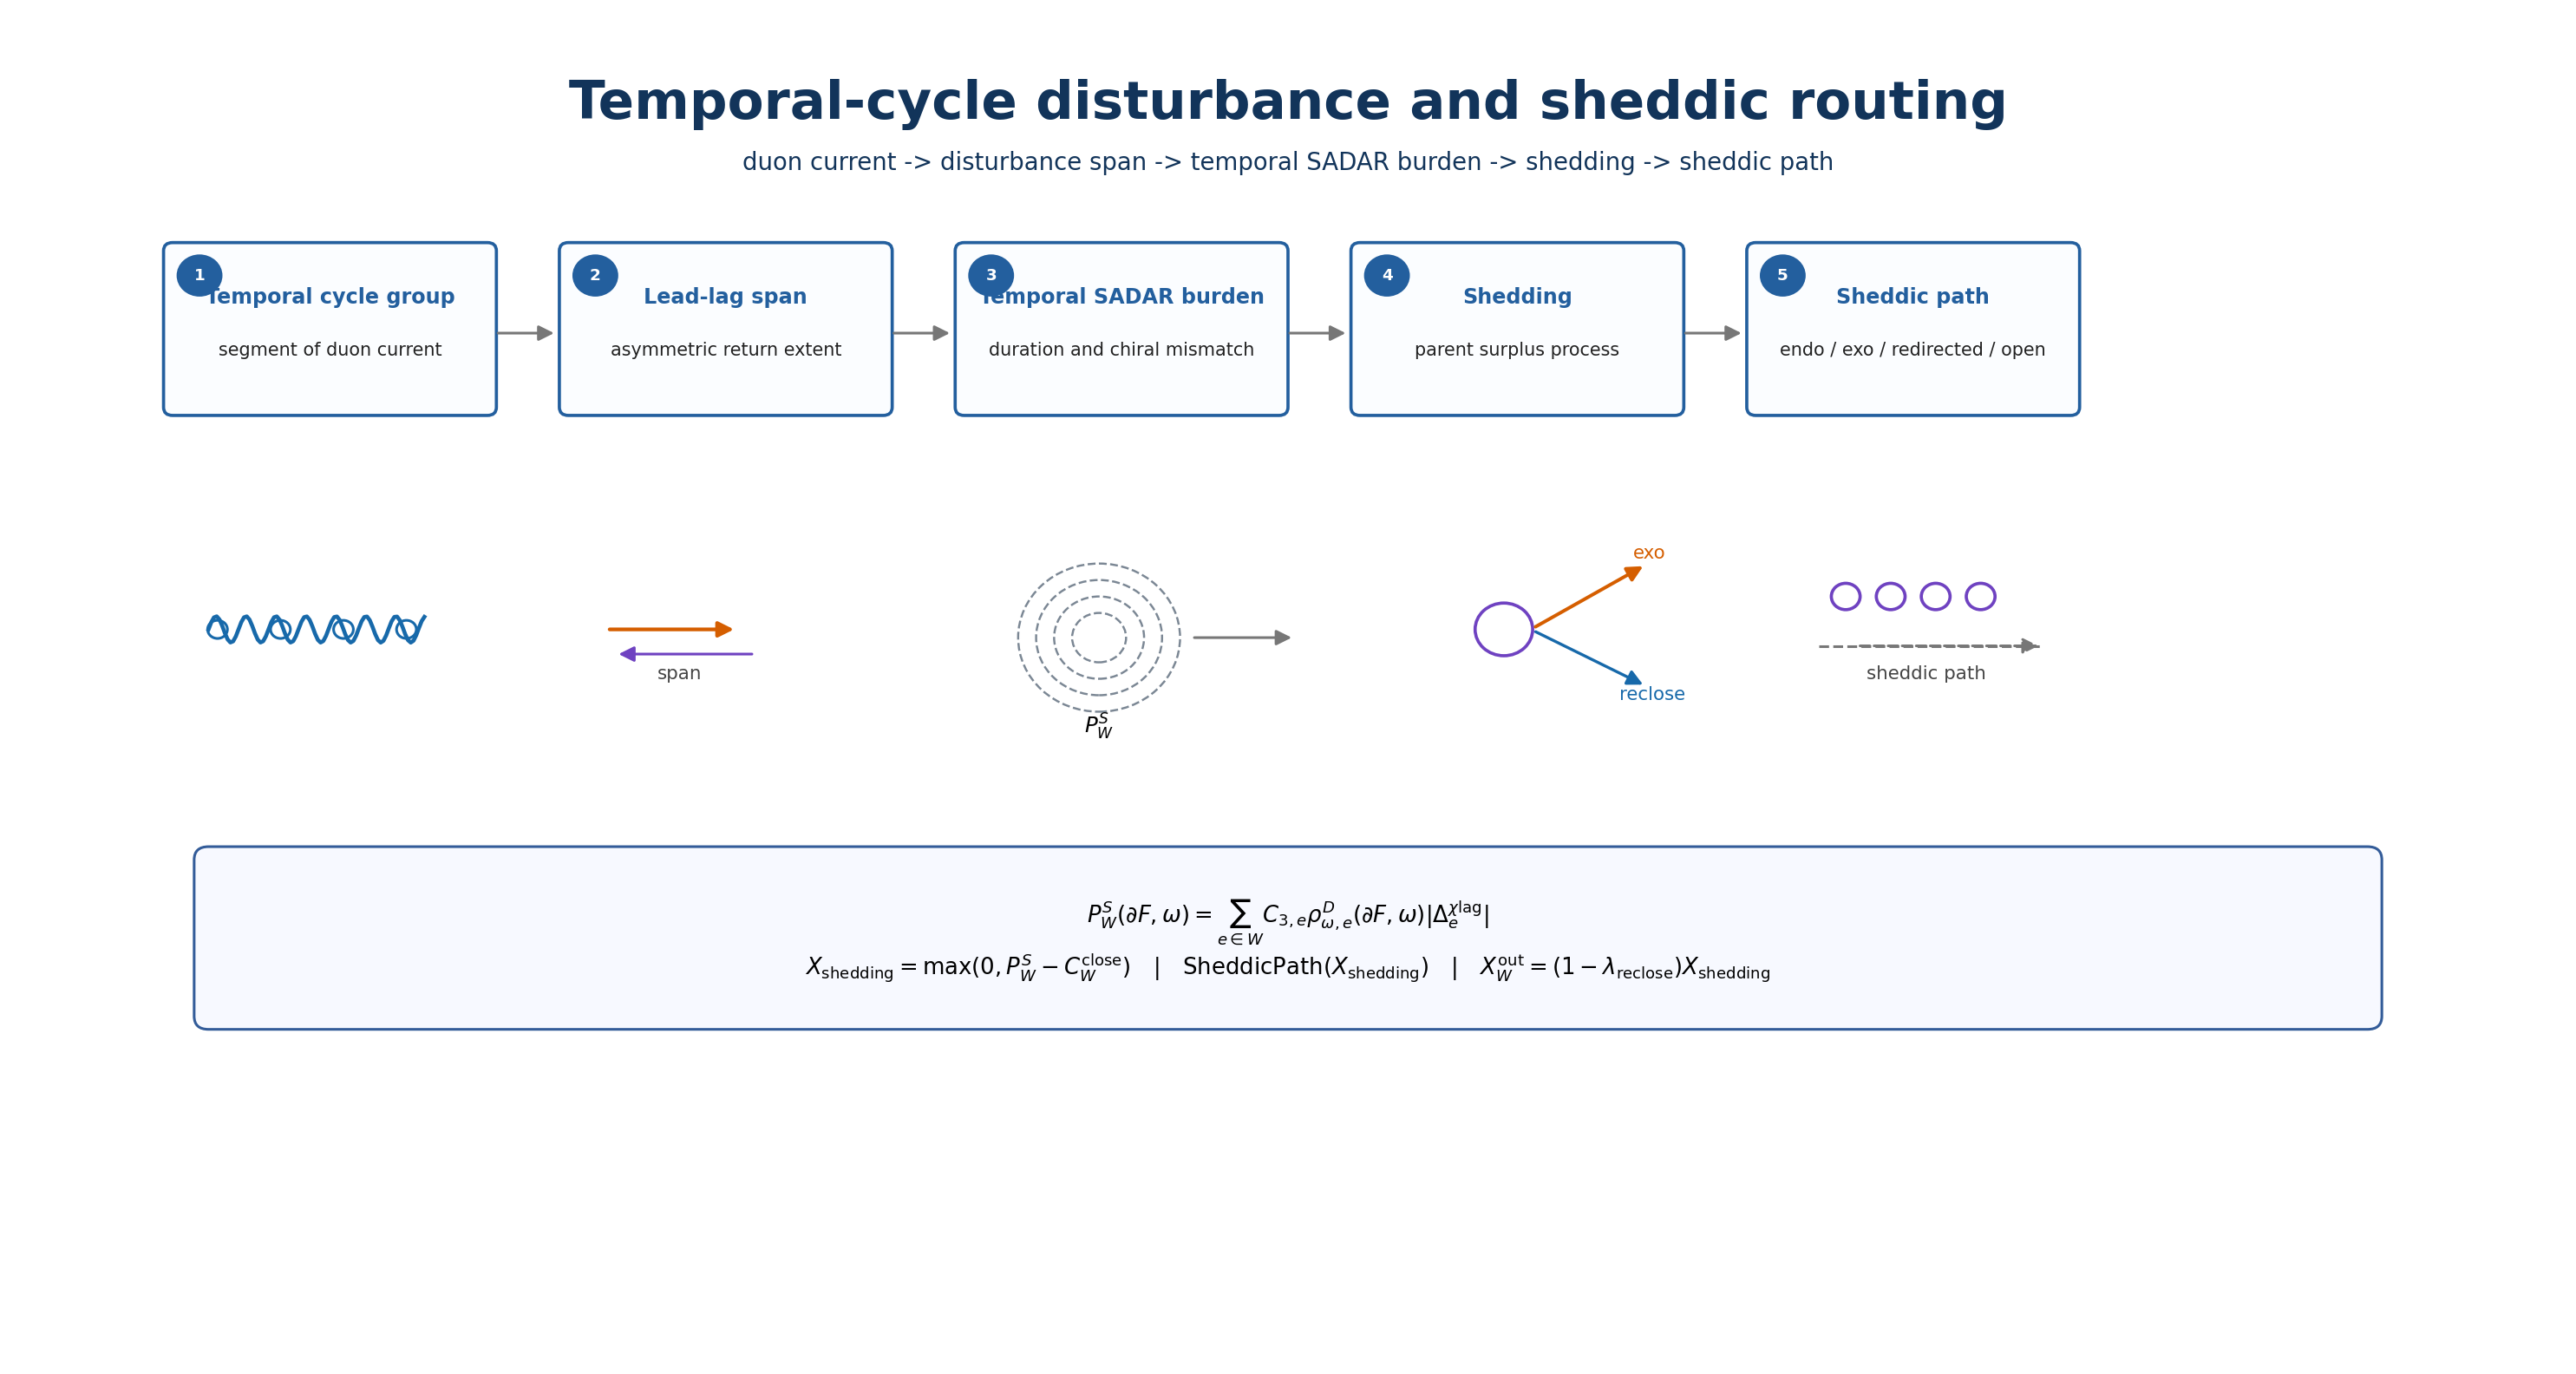
\includegraphics[width=0.96\linewidth]{figures_jpg/cycle_disturbance_shedding.png}
\caption{Temporal cycle lead--lag disturbance and shedding. On the declared boundary/window $B=(\partial F,\omega)$, the schematic $\Delta_e^{\chi\mathrm{lag}}$ denotes the signed lag accessor $\Delta\chi_e^{\mathrm{lag}}(B)$; the absolute-value bars take its magnitude.}
\label{fig:v39-cycle-disturbance-shedding}
\end{figure}

\aodprovenance{\eqnref{eq:closure-certificate},
\eqnref{eq:return-identity},
\eqnref{eq:beat-reclosure},
\eqnref{eq:cumulative-closure-counts},
\eqnref{eq:closure-phase-window},
\eqnref{eq:duon-current},
\eqnref{eq:aod-wavelet-continuation},
\eqnref{eq:returned-duration},
\eqnref{eq:temporal-sadar-burden},
\eqnref{eq:shedding-excess},
\eqnref{eq:sheddic-path},
\eqnref{eq:shed-continuation-witness},
\eqnref{eq:recipient-event-lattice},
\eqnref{eq:sadar-attention-vector},
\eqnref{eq:entropic-duon-current},
\eqnref{eq:sadar-field},
\appref{app:wave},
\appref{app:curling-curls}.}

\subsection{Seat compatibility and shell/enclosure routing}\label{sec:seat-shell-enclosure-routing}

\subsubsection{Even sequence}\label{subsec:support-enclosure-even-sequence}

The even sequence separates the current-side double form, the inner enclosure, and the outer enclosures.

\subsubsection{E2 duon}\label{subsec:e2-duon}

In seat-compatibility routing, $E_2$ and $E_2^0$ invoke the canonical Duon
support owned in \secref{subsec:duon} (\eqref{eq:duon-current}).

\subsubsection{E2$^{\pm}$ duad}\label{subsec:e2-duad}

In seat-compatibility routing, $E_2^{\pm}$ invokes the canonical same-current
Duad seating state owned in \secref{subsec:duad} (\eqref{eq:duad-same-current}).

\subsubsection{E4 tetron}\label{subsec:e4-tetron}

\[
E_4=\mathrm{tetron}.
\]

Tetron is the default inner enclosure with four seats.

\subsubsection{Outer enclosures}\label{subsec:outer-enclosures}

A support enclosure is an outer even enclosure available to shell/enclosure routing:

\[
\mathsf{C}_{2m}=\text{support enclosure of order }2m,\qquad m\ge3.
\]

\subsubsection{Hexon}\label{subsec:hexon}

\[
\mathsf{C}_6=\mathrm{hexon}.
\]

Hexon is the first outer enclosure because the hinge triad supplies left/right threefold closure: $\mathsf{H}_3+\mathsf{H}_3=6$.

\subsubsection{Octon}\label{subsec:octon}

\[
\mathsf{C}_8=\mathrm{octon}.
\]

\subsubsection{Decon}\label{subsec:decon}

\[
\mathsf{C}_{10}=\mathrm{decon}.
\]

\subsubsection{Higher even enclosures}\label{subsec:higher-even-enclosures}

Higher even enclosures continue the outer sheddic path sequence:

\[
\mathsf{C}_{2n},\qquad n>5.
\]

Outer enclosures are retained forms of sheddic paths. Hexon is the first outer enclosure; octon and decon are higher sheddic path forms; $\mathsf{C}_{2n}$ records the higher even sequence.

\subsubsection{Filled shared enclosure}\label{subsec:filled-shared-enclosures}

A filled shared enclosure has

\[
m:m:0::2m,\qquad m\ge3.
\]

\subsubsection{Closure excess}\label{subsec:support-enclosure-sadar-closure}

For a support-enclosure declaration $\mathcal{C}=a:b:c::L$ on $B=(\partial F,\omega)$, shell/enclosure routing carries the already-declared sheddic excess on the available route $\mathcal{C}$. The routed closure excess is

\begin{equation}\label{eq:support-enclosure-excess}
X_{\mathcal{C}}(B)=\operatorname{route}_{\mathcal{C}}(X_{\mathrm{shedding}}(B)).
\end{equation}

The value and placement of $X_{\mathcal{C}}$ determine local rebalancing, exoshedding, endoshedding, or redirected support routing.

\subsubsection{Seat-compatible retention duration}\label{subsec:support-enclosure-retention-condition}

For a support-enclosure declaration $\mathcal{C}=a:b:c::L$, write

\begin{equation}\label{eq:support-enclosure-retention}
\mathrm{TTL}_{\mathcal{C}}(\partial F,\omega)=\text{retained tick duration available for seat-compatible SADAR rebalancing}.
\end{equation}

This is distinct from $\rho^D_{\omega,ij}(B)$, the window-clipped duration participation for a channel.
Retention on the declared window is $\mathrm{TTL}_{\mathcal{C}}(\partial F,\omega)\ge|\omega|$. If $\mathrm{TTL}_{\mathcal{C}}(\partial F,\omega)<|\omega|$, the sheddic path continues through re-entry, reclosure, or decay status before the window closes.

\begin{figure}[H]
\centering
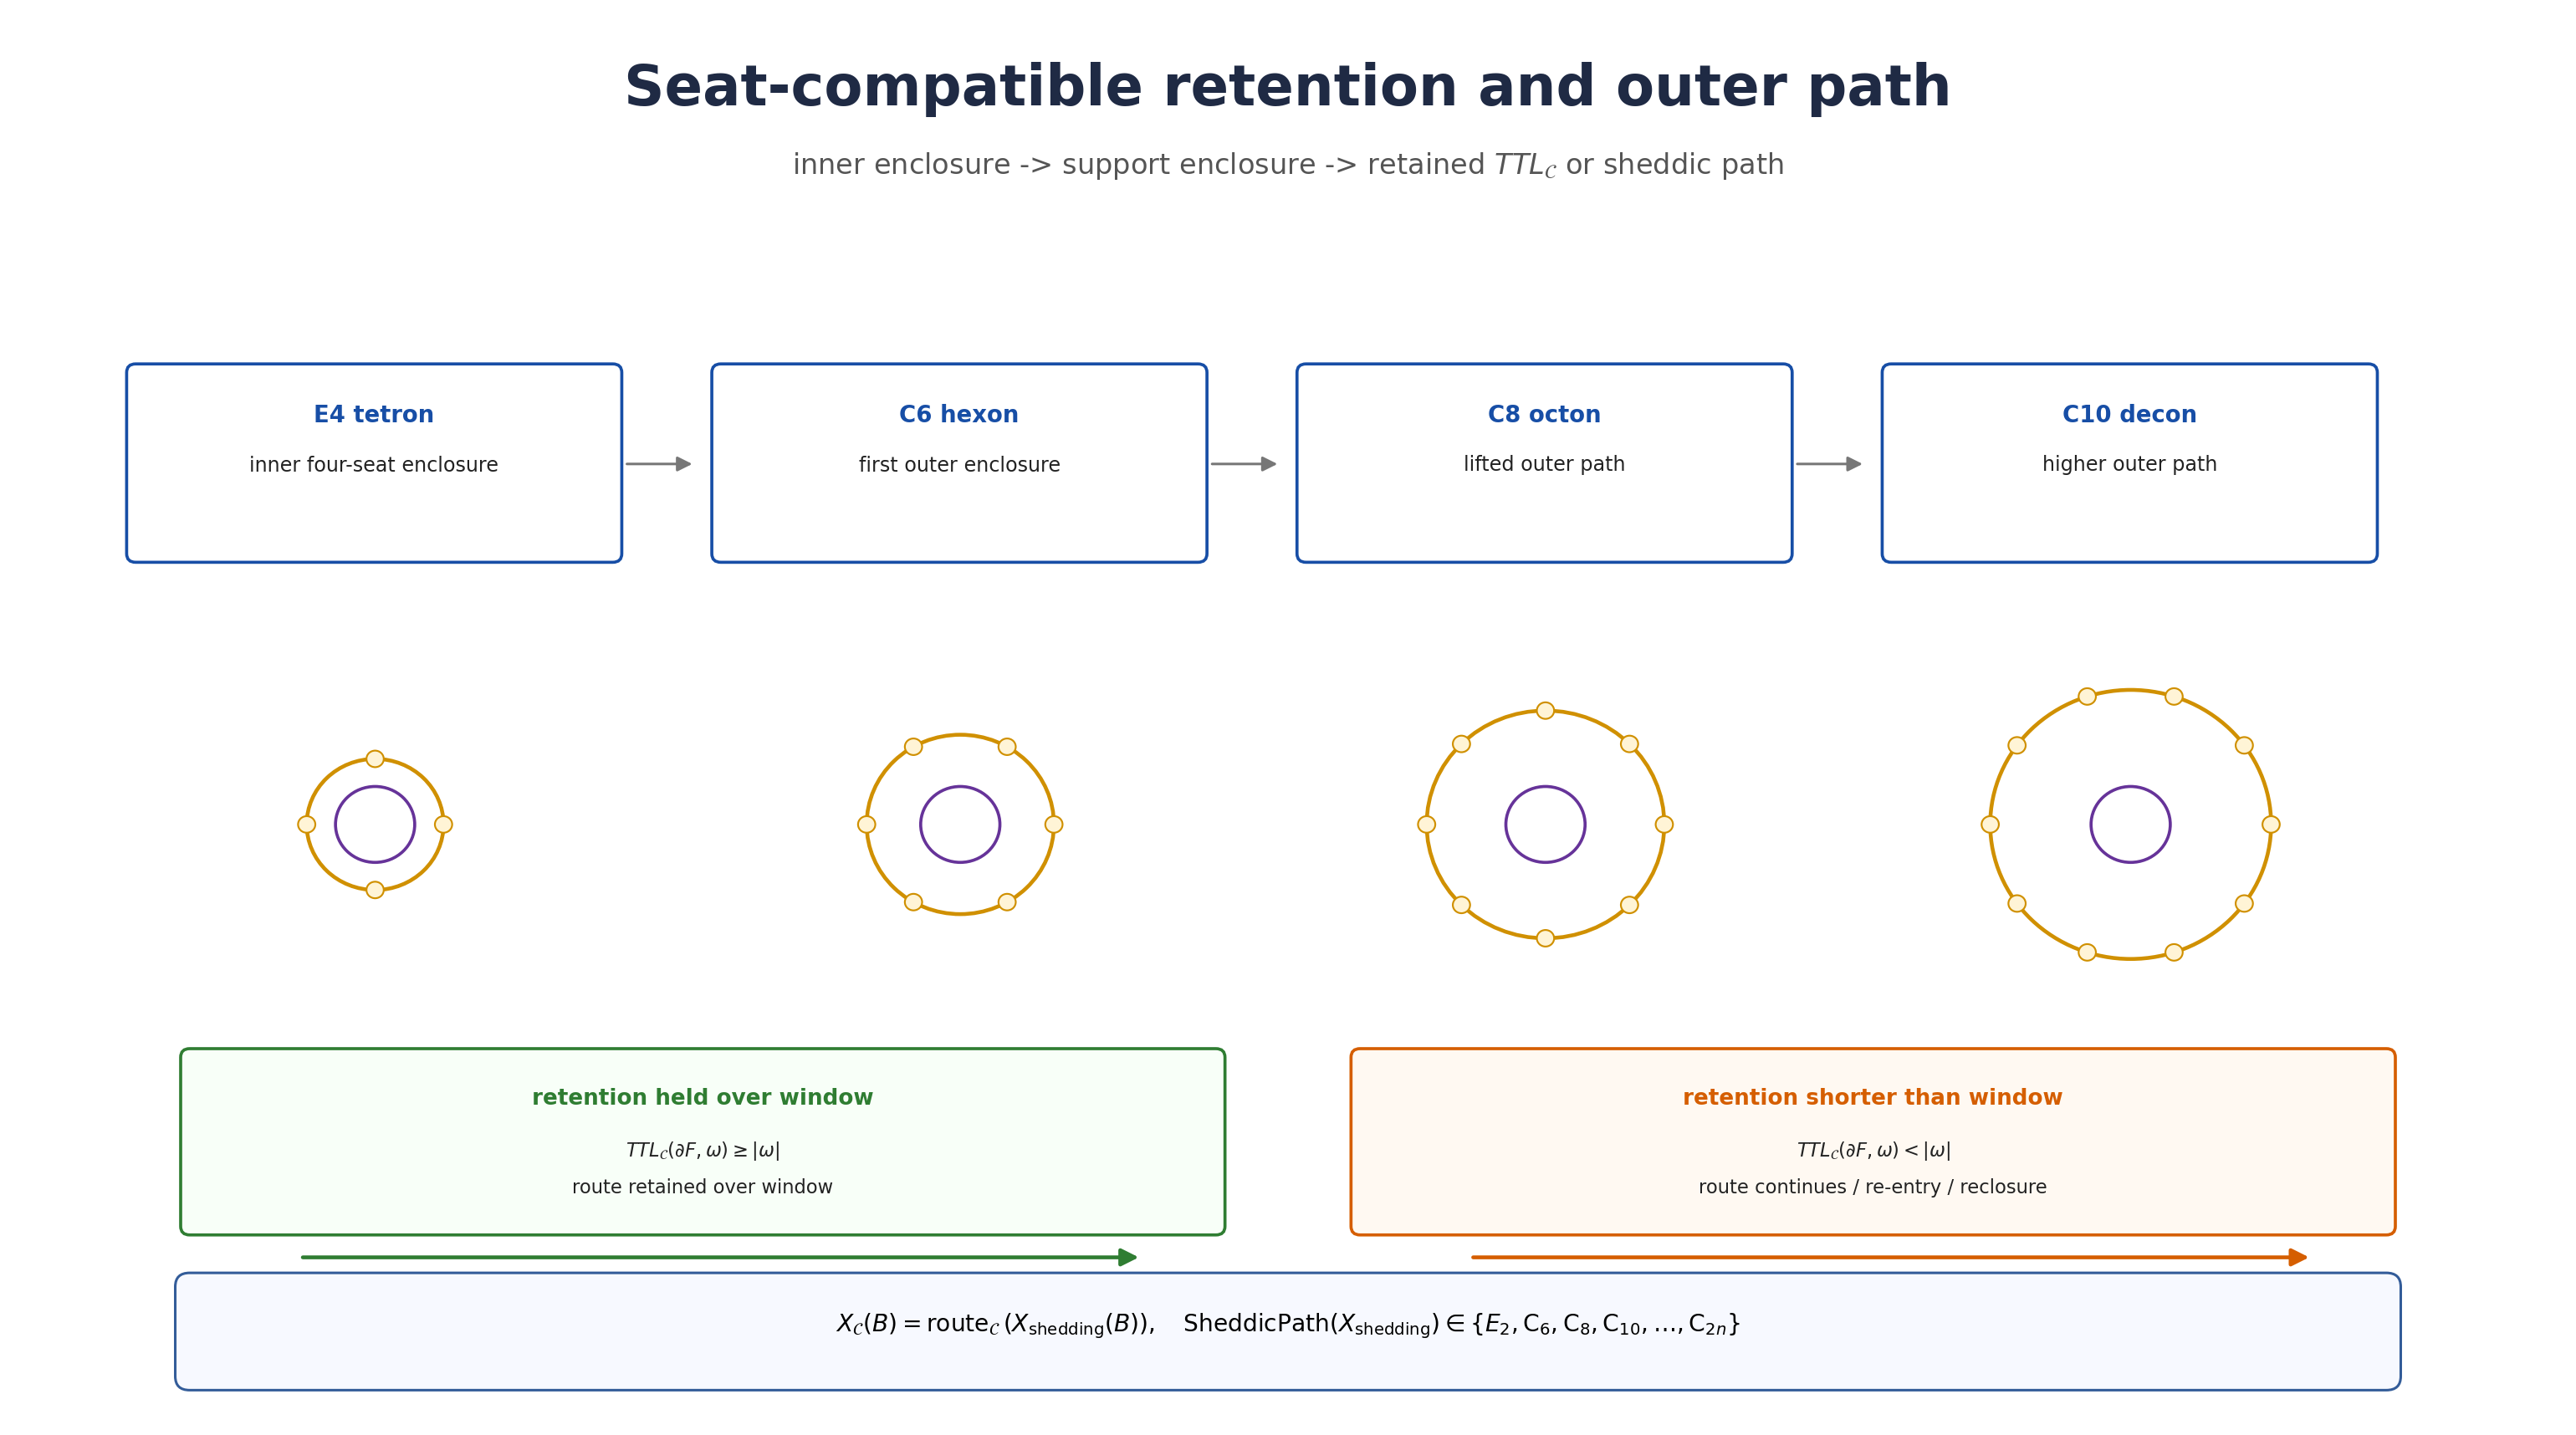
\includegraphics[width=0.96\linewidth]{figures_jpg/support_enclosure_retention.png}
\caption{Seat compatibility and support-retention duration for sheddic paths.}
\label{fig:support-enclosure-retention}
\end{figure}

\subsubsection{Coord-0 grouping}\label{subsec:coord-zero-support-enclosure-grouping}

At coordinate $0$, write coord-0 shell-stack declarations as

\[
0\mid-::Z:A:0:L\langle a:b:c::L\rangle.
\]

For filled support-enclosure grouping,

\[
0\mid-::Z:A:0:2m\langle m:m:0::2m\rangle.
\]

Define the cumulative group boundary

\[
\Gamma_m=\sum_{k=3}^m2k=m(m+1)-6,\qquad\Gamma_2=0.
\]

Then $\Gamma_{m-1}<Z\le\Gamma_m$ selects the coord-0 support-enclosure group.

\aodprovenance{\eqnref{eq:sadar-field},
\eqnref{eq:support-enclosure-excess},
\eqnref{eq:support-enclosure-retention},
\appref{app:curling-curls}.}

\subsection{Shell paths}\label{sec:shell-paths}

\subsubsection{Shell-path closure references}\label{subsec:shell-path-closure-references}

Shell paths retain channel pressure \eqref{eq:b-scoped-channel-pressure} and
flux \eqref{eq:b-scoped-flux}. Their closure controls are in
\appref{app:combinatorics-rd-tests} and
\appref{app:path-complexity-quarantine}.

\subsection{Fusion closure and chain reclosure}\label{sec:fusion-closure-chain-reclosure}

\subsubsection{Fusion closure}\label{subsec:fusion-closure}

Fusion is branch/hinge/branch closure of admitted curling-curl support forms. For admitted forms $F$ and $G$, define

\begin{equation}\label{eq:fusion-closure}
\operatorname{Fuse}_B(F,G):=\operatorname{Close}_B(\hat{F}\;\mu\;\hat{G}),
\end{equation}

where $\hat{F}=\operatorname{Compress}(F)$ and $\hat{G}=\operatorname{Compress}(G)$. Closed forms fuse; exposed fragments do not.
The inherited fusion operator consumes closed or reclosed admitted inputs.
Each input compression must have its complete inner construction and certificate
bound before consumption. The outer certificate binds both compressed inputs;
an incomplete compression or an open proposal is outside this operator's domain.

The branch/hinge/branch fusion duration is

\begin{equation}\label{eq:fusion-branch-hinge-duration}
RD_{\mathrm{fuse}}(F,G;B)=\Pi^-_{\hat{F}}(B)+H_{\mu,\hat{F},\hat{G}}(B)+\Pi^+_{\hat{G}}(B).
\end{equation}

For a closure rung,

\begin{equation}\label{eq:fusion-ladder-rung}
C^{\mathrm{ret}}_{n+1}=\operatorname{Close}_{B_{n+1}}(\hat{F}_n\;\mu\;\hat{G}_n).
\end{equation}

The rung residual is

\begin{equation}\label{eq:fusion-rung-residual}
S_{n+1}=P^D_{n+1}-C_{\mathrm{close},n+1}.
\end{equation}

If $S_{n+1}>0$, the rung is surplus-producing; if $S_{n+1}=0$, its scalar residual is neutral; if $S_{n+1}<0$, it is deficit/open. Every claimed closure also requires its independent trace certificate. The sheddic surplus is

\begin{equation}\label{eq:fusion-rung-shedding-surplus}
X_{\mathrm{shedding},n+1}=\max(0,S_{n+1}).
\end{equation}

\subsubsection{Exoshedding lift}\label{subsec:exoshedding-lift}

Exoshedding routes surplus support outside the current closure. At scope $B_r$, nonzero $X_{\mathrm{exo},r}$ supplies proposed lifted support

\begin{equation}\label{eq:exoshedding-lift}
K^{r+1}_{\mathrm{prop}}=\operatorname{Lift}_{B_r\to B_{r+1}}(X_{\mathrm{exo},r}).
\end{equation}

The construction trace admits it by

\begin{equation}\label{eq:lifted-support-admission}
K^{r+1}_{\mathrm{prop}}\xrightarrow{\,HT(K;B_{r+1})\,}K^{r+1}_{\mathrm{adm}}(B_{r+1}).
\end{equation}

Higher-scope fusion closes the admitted lifted support:

\begin{equation}\label{eq:higher-scope-fusion}
C^{\mathrm{ret}}_{r+1}=\operatorname{Close}_{B_{r+1}}(\hat{F}_r\;\mu\;K^{r+1}_{\mathrm{adm}}(B_{r+1})).
\end{equation}

Thus exoshedding supplies lifted support; fusion closes it.

\subsubsection{Link-closure ladder}\label{subsec:link-closure-ladder}

Chain reclosure is iterated higher-scope fusion over admitted supports routed by exoshedding. A local adjacent link closure is

\begin{equation}\label{eq:link-closure-ladder}
L_{i,i+1}=\operatorname{Close}_{B_{i,i+1}}(\hat{F}_i\;\mu\;\hat{F}_{i+1}).
\end{equation}

Its residual is

\begin{equation}\label{eq:link-closure-residual}
\Delta_{\mathrm{link}}=P^D_{\mathrm{link}}-C_{\mathrm{close,link}},\qquad X_{\mathrm{shedding},\mathrm{link}}=\max(0,\Delta_{\mathrm{link}}).
\end{equation}

\aodprovenance{\secref{subsec:curling-curl-support-forms}, \secref{subsec:sheddic-path}, \eqnref{eq:branch-hinge-rd}.}

\subsection{Fractal Field Ring Gate}\label{subsec:fractal-field-ring-gate}

\aodnoteblock{Scope}{A fractal field ring gate is a declared recurrence motif on $B=(\partial_TF,\omega)$.}

Declare

\begin{equation}\label{eq:frg-scope}
\mathfrak{a}\subset\mathcal{A}^{\mathrm{ret}}_8,\qquad B=(\partial_TF,\omega).
\end{equation}

The AF recurrence is typed here: the distinctions are declared in \eqnref{eq:frg-distinctions}; the relations are declared in \eqnref{eq:frg-ring-adjacency}--\eqnref{eq:frg-return-relation}; the retained relation family is the FRG; $\SADARop_B$ forms the A$\Omega$ value.

\subsubsection{Distinctions}\label{subsec:frg-distinctions}

Declare

\begin{equation}\label{eq:frg-distinctions}
D_{\mathrm{FRG}}=(\mathfrak{a},B,V_N,I,G).
\end{equation}

with

\[
V_N=\{0,1,\dots,N-1\},\qquad R_{\mathrm{ring}}\subset F,
\]

\[
\partial_TR_{\mathrm{ring}}=\text{the tesseract-admissible boundary induced on }R_{\mathrm{ring}},
\]

\[
I\subseteq V_N,\qquad G=\{g_i:i\in I\},\qquad g_i\in\partial_TR_{\mathrm{ring}},
\]

\[
k\in K_{\mathrm{bin}}.
\]

\subsubsection{Relations}\label{subsec:frg-relations}

The ring adjacency relation is

\begin{equation}\label{eq:frg-ring-adjacency}
E_N=\{(i,i+1\bmod N),(i,i-1\bmod N):i\in V_N\}.
\end{equation}

The returned-current relation is

\begin{equation}\label{eq:frg-return-relation}
E_{\mathrm{return}}\subseteq I\times I.
\end{equation}

Under the adjacent-only restriction,

\begin{equation}\label{eq:frg-adjacent-only-condition}
(i,j)\in E_{\mathrm{return}}\Rightarrow(i,j)\in E_N.
\end{equation}

Gate-to-bin and cross-return path relations are written directly as

\[
\gamma:g_i\leadsto k,\qquad\gamma:g_i\leftrightarrow g_j\leadsto k.
\]

The retained path-cycle carried by $\gamma$ is $C_{\gamma}$.

\paragraph{Retained relation, admission and model.}

\begin{equation}\label{eq:frg-admission-order}
D_{\mathrm{FRG}}\longrightarrow R^{\mathrm{ret}}_{\mathrm{FRG}}\longrightarrow K_{\mathrm{FRG,adm}}(B,i;\mathrm{cert})\longrightarrow(K_{\mathrm{bin}},\kappa,\lambda_{\mathcal{Y}}).
\end{equation}

The retained ring adjacency and return paths carry distinction identities.
After \eqref{eq:motif-admission}, choose
$\kappa:K_{\mathrm{bin}}\to\mathbb{Q}$, $\kappa_k=\kappa(k)$, and the
value map $\lambda_{\mathcal{Y}}$. The sums consume paths committed through
the current cut; response follows at the next transition.

\subsubsection{Gate contribution}\label{subsec:frg-gate-contribution}

For a declared gate $g_i$, define the bin contribution

\begin{equation}\tag{RG1}\label{eq:frg-gate-contribution}
S_k^{(i)}=\sum_{t\in\omega}\sum_{\gamma:g_i\leadsto k}\kappa_k\,\SADARop_{B|t}(C_{\gamma}).
\end{equation}

\subsubsection{Independent gate-sum value}\label{subsec:frg-independent-gate-sum}

The independent gate-sum value is

\begin{equation}\tag{RG2}\label{eq:frg-independent-gate-sum}
T_k^0=\sum_{i\in I}S_k^{(i)}.
\end{equation}

For two gates,

\begin{equation}\tag{RG3}\label{eq:frg-independent-two-gate}
T_k^0=S_k^{(a)}+S_k^{(b)}.
\end{equation}

\subsubsection{Cross-return contribution}\label{subsec:frg-cross-return-contribution}

For a returned-current pair $(i,j)\in E_{\mathrm{return}}$, define

\begin{equation}\tag{RG4}\label{eq:frg-cross-return-contribution}
C_{ij,k}^{\times}(B)=\sum_{t\in\omega}\sum_{\gamma:g_i\leftrightarrow g_j\leadsto k}\kappa_k\,\SADARop_{B|t}(C_{\gamma}).
\end{equation}

For the two-gate specialization with
$E_{\mathrm{return}}=\{(a,b)\}$,

\begin{equation}\tag{RG5}\label{eq:frg-cross-return-two-gate}
C_{ab,k}^{\times}(B)=\sum_{t\in\omega}\sum_{\gamma:g_a\leftrightarrow g_b\leadsto k}\kappa_k\,\SADARop_{B|t}(C_{\gamma}).
\end{equation}

\subsubsection{Recurrent ring value}\label{subsec:frg-recurrent-ring-value}

The recurrent ring value is

\begin{equation}\tag{RG6}\label{eq:frg-recurrent-ring-value}
T_k^{\times}=T_k^0+\sum_{(i,j)\in E_{\mathrm{return}}}C_{ij,k}^{\times}(B).
\end{equation}

Under the specialization of \eqnref{eq:frg-cross-return-two-gate},

\begin{equation}\tag{RG7}\label{eq:frg-recurrent-two-gate}
T_k^{\times}=T_k^0+C_{ab,k}^{\times}(B).
\end{equation}

\subsubsection{Field-ring identity}\label{subsec:frg-identity}

The field-ring identity is

\begin{equation}\tag{RG8}\label{eq:frg-identity}
T_k^{\times}-T_k^0=\sum_{(i,j)\in E_{\mathrm{return}}}C_{ij,k}^{\times}(B).
\end{equation}

Under the specialization of \eqnref{eq:frg-cross-return-two-gate},

\begin{equation}\tag{RG9}\label{eq:frg-identity-two-gate}
T_k^{\times}-T_k^0=C_{ab,k}^{\times}(B).
\end{equation}

(The exact-fixture residual tag $\mathrm{RG10}$ belongs to the downstream Manual fixture layer.)

\subsubsection{FRG value package}\label{subsec:frg-value-package}

The compact FRG value package is

\begin{equation}\tag{RG11}\label{eq:frg-value-package}
\mathcal{V}_{\mathrm{FRG}}=(\mathfrak{a},B,R_{\mathrm{ring}},\partial_TR_{\mathrm{ring}},V_N,E_N,I,G,K_{\mathrm{bin}},\kappa,E_{\mathrm{return}},\lambda_{\mathcal{Y}}).
\end{equation}

The declared value map is

\begin{equation}\tag{RG12}\label{eq:frg-value-map}
\lambda_{\mathcal{Y}}:(T_k^{\times})_{k\in K_{\mathrm{bin}}}\mapsto\mathcal{Y}.
\end{equation}

\aodremark{FRG supplies gated recurrent cross-return; fusion closes admitted support.}

\subsection{Field dynamics}\label{sec:field-dynamics}

\subsubsection{Field-fluid regime}\label{subsec:field-fluid-regime}

Field dynamics is the A$\Omega$D calculation of retained field, current-cycle, background-continuation, and shell-support participants on declared $B=(\partial_TF,\omega)$. A field-fluid regime is the local declaration in which those participants couple through finite SADAR capacity. For a moving or nested cell boundary, write

\[
B_c|t=(\partial_TR_c(t),\omega_c|t).
\]

The retained cycle family is

\[
\mathcal{C}_c(t)=\mathcal{C}_{\mathrm{field},c}\cup\mathcal{C}_{\mathrm{current},c}\cup\mathcal{C}_{\mathrm{bg},c}\cup\mathcal{C}_{\mathrm{shell},c}.
\]

Here

\[
C_J=\text{retained current-cycle participant},\qquad J^D=\text{accumulated current value}.
\]

\subsubsection{Support-resolution model}\label{subsec:cycle-beat-resolution-gate}

Let

\[
\mathcal{C}_{a,r,\Sigma}=\operatorname{cycle}\langle a,r\rangle(\Sigma_{\mathrm{support}}),
\]

where $\Sigma_{\mathrm{support}}$ is the declared support-expression family,
with structural support multiplicity $N_{\mathrm{support}}(a,r,\Sigma;B)$
defined by \eqref{eq:beat-count}.
The monitored reflection-duration accessor is selected by the declared rule

\[
RD_{\mathrm{mon}}(a,r,\Sigma;B)=\max_{C_u\in\mathcal{C}_{a,r,\Sigma}}RD_{\AO}(C_u;B).
\]

Resolution is chosen by a declared coarseness order $\preceq_{\mathrm{coarse}}$. Tie-breakers are declared before application. The selected $q$ is the coarsest resolution among already admitted candidates under $\preceq_{\mathrm{coarse}}$ after declared tie-breakers. No measured residual or score enters this gate.

\subsubsection{Medium declaration and field count}\label{subsec:medium-declaration-field-count}

Declare $N_{\mathrm{candidate},c},N_{\mathrm{support},c}\in\mathbb{Z}_{\ge0}$, $\mathcal{K}^{\mathrm{raw}}_c\in\mathbb{Q}_{\ge0}$, and $\bar{k}_F,\bar{\rho}^D_F\in\mathbb{Q}_{>0}$ before application. The raw maximum supported field count is

\[
N^{\max,0}_{F,c}=\min(N_{\mathrm{candidate},c},N_{\mathrm{support},c},\lfloor\frac{\mathcal{K}^{\mathrm{raw}}_c}{\bar{k}_F}\rfloor,\lfloor\frac{|\omega_c|}{\bar{\rho}^D_F}\rfloor).
\]

Subject to actual recurrent member admission, the retained field family is then bounded as

\[
F_{B_c}=\{F_1,\dots,F_{n_F(c)}\},\qquad n_F(c)\le N^{\max,0}_{F,c}.
\]

A gas/fluid classifier is a declaration on $B_c$, not an external material label. Chiral flip, background-continuation jitter, slosh, semi-coupling, and lead-lag are boundary-current features of the declared regime.

\aodremark{A field-fluid regime may distinguish locally seated, unresolved-jitter, pending, and sheddic chiral events by declared boundary status.}

\subsubsection{Nested boundary and inter-layer SADAR coupling}\label{subsec:interlayer-sadar-coupling}

For nested boundaries

\[
R_0\subset R_1\subset\cdots\subset R_m,\qquad B_{\ell}=(\partial_TR_{\ell},\omega_{\ell}),
\]

the inter-layer coupling value is

\[
G^{\mathfrak{S}}_{\ell\to m}(B)=\sum_{(u,v)\in E^{\mathfrak{S}}_{\ell,m}(B)}\SADARop_B(C_u,C_v).
\]

Range-prioritized coupling orders admissible $E^{\mathfrak{S}}_{\ell,m}(B)$ by the declared boundary range before summation. When a magnitude is needed, use the declared magnitude functional

\[
J^{D,\mathrm{try}}_{r,c}=\sum_{(u,v)\in E_r(B_c)}\|\SADARop_{B_c}(C_u,C_v)\|_{\mathrm{decl}}.
\]

\subsubsection{Capacity residual and exoshedding lift}\label{subsec:capacity-residual-exoshedding-lift}

Declare the capacity residual $\Delta^{\mathrm{cap}}_{\ell}=P^D_{\ell}-C^{\mathrm{cap}}_{\ell}$.
The separate closure residual, surplus and route partition use
\eqref{eq:closure-residual}, \eqref{eq:shedding-excess} and
\eqref{eq:shedding-route-partition} on $B_{\ell}$.
For $X_{\mathrm{exo},\ell}>0$, apply \eqref{eq:exoshedding-lift},
then \eqref{eq:lifted-support-admission} before
\eqref{eq:higher-scope-fusion}. Capacity and closure compatibility retain
their distinct operands.

\subsubsection{FRG-mediated cross-return in nested boundaries}\label{subsec:frg-nested-boundary}

A ring-gated layer instantiates \eqref{eq:frg-distinctions} and
\eqref{eq:frg-admission-order} with its own
$N_{\ell},I_{\ell},G_{\ell},K_{\mathrm{bin},\ell},\kappa_{\ell},E_{\mathrm{return},\ell}$.
Its cross terms and recurrent value are
\eqref{eq:frg-cross-return-contribution} and \eqref{eq:frg-recurrent-ring-value}
on $B_{\ell}$. FRG supplies gated cross-return; the preceding lift and fusion
construct the higher closure, and their iteration gives chain reclosure.

\begin{figure}[H]
\centering
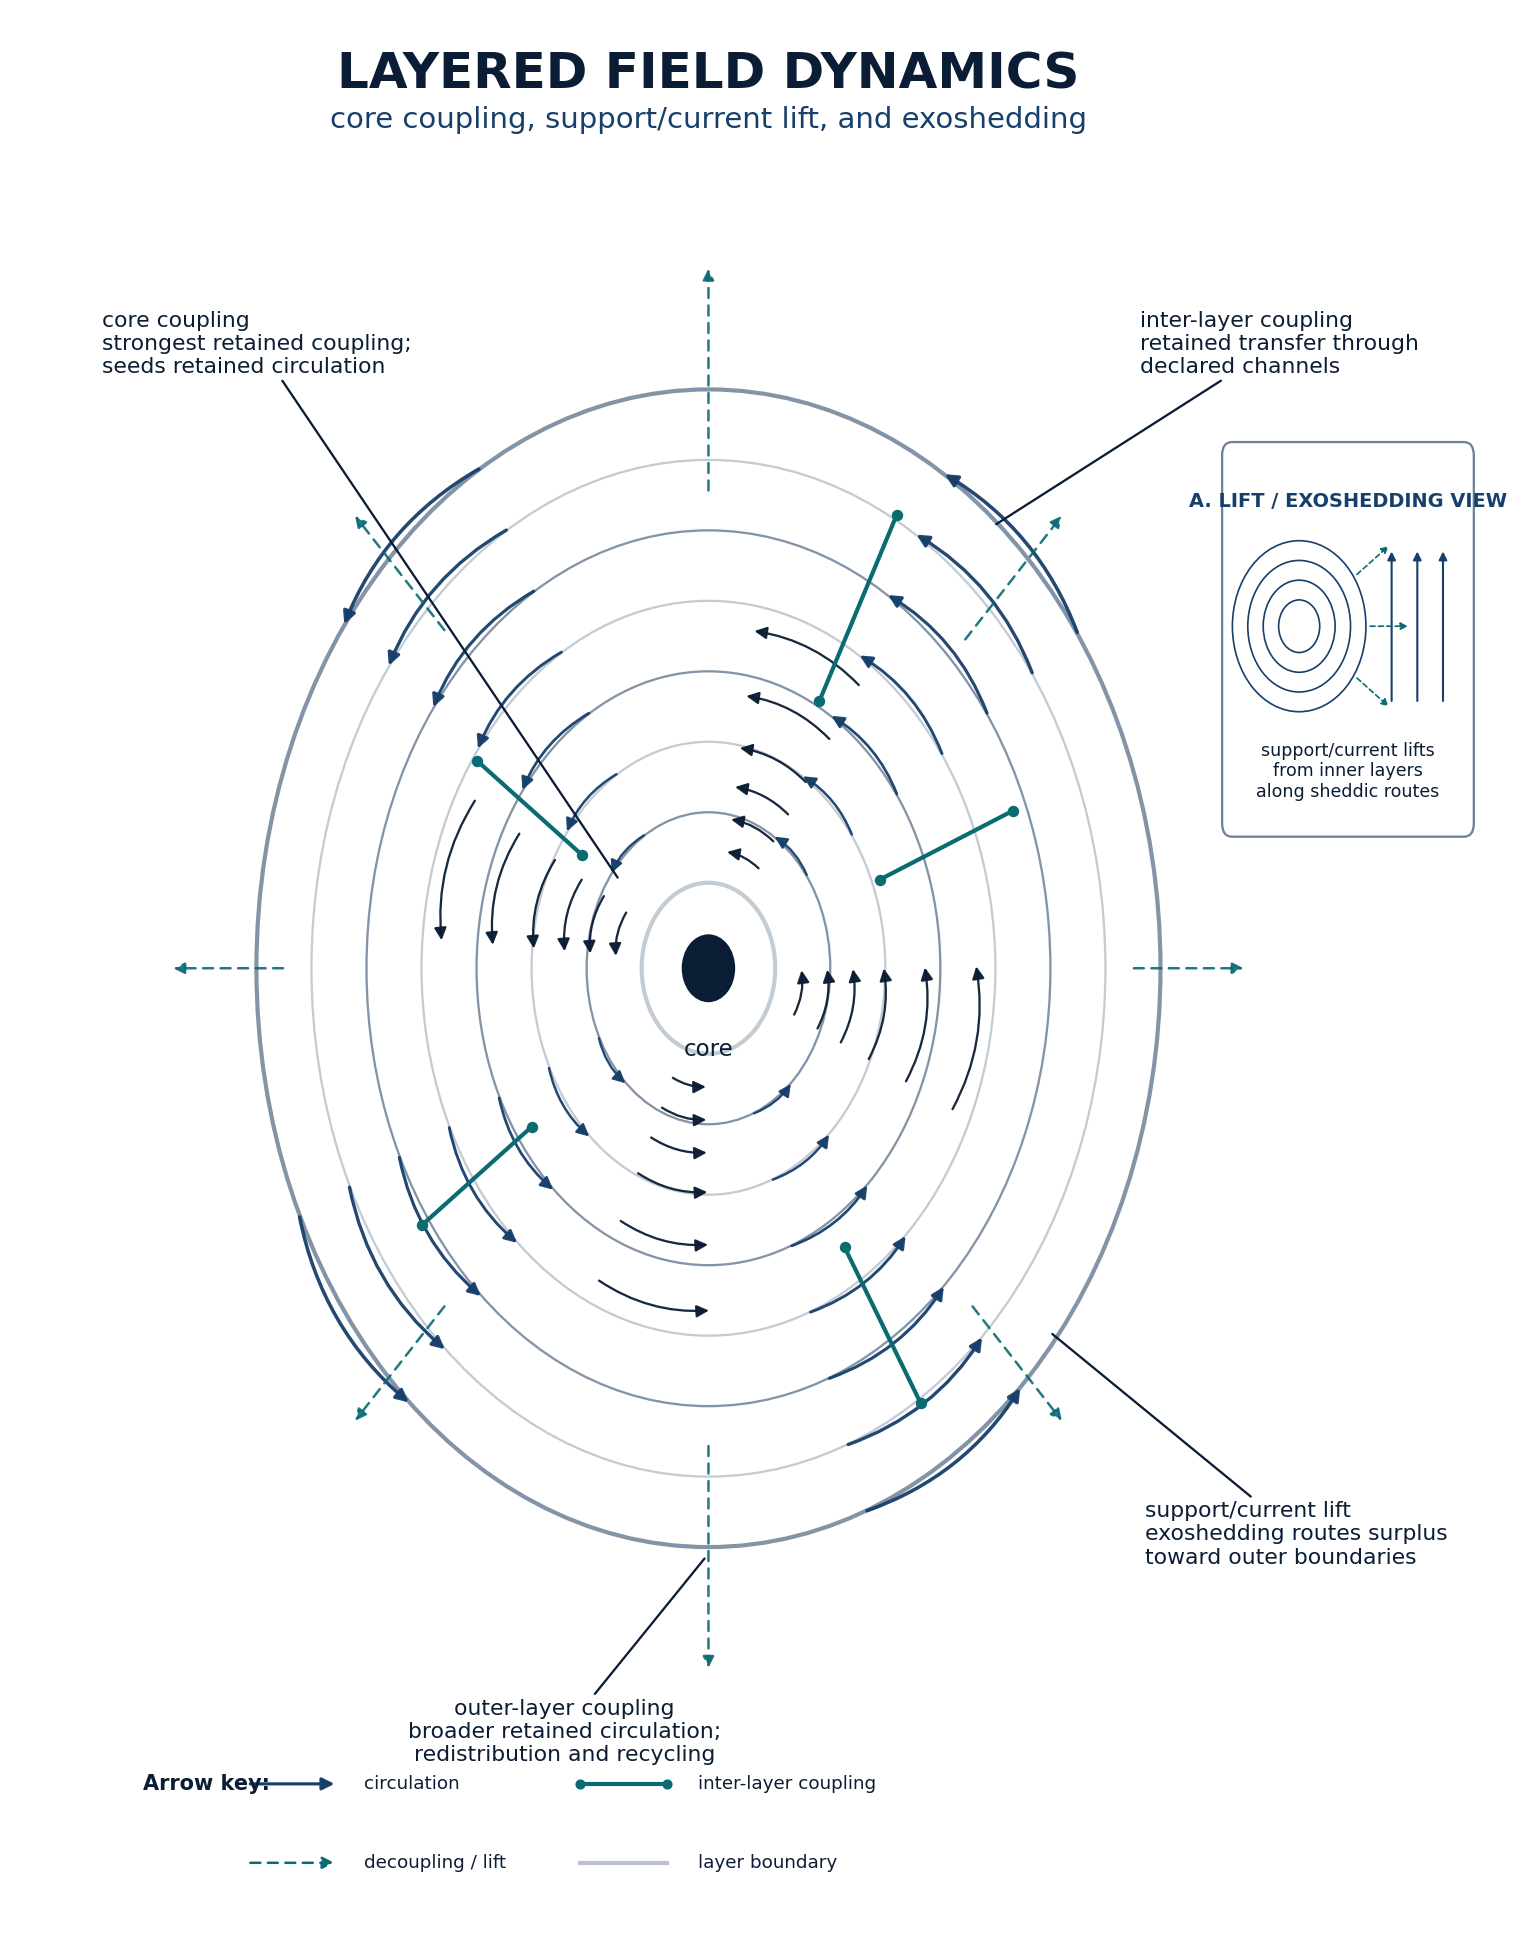
\includegraphics[width=0.82\linewidth]{figures_jpg/field_dynamics_layered_main.png}
\caption{Layered field dynamics. Boundaries separate layers; same-sense circulation remains on each layer; coupling arrows cross declared inter-layer channels; decoupling/lift arrows indicate exoshedding after closure surplus.}
\label{fig:field-dynamics-layered}
\end{figure}

\subsubsection{Finite SADAR moving-boundary dictionary}\label{subsec:finite-sadar-moving-boundary-dictionary}

On $B_c|t$, substitute $\varphi_e=\SADARop(C_e)$ into
\eqref{eq:slice-flux}; sum with \eqref{eq:window-current} and retain the
crossing/sweep/shedding split of \eqref{eq:moving-boundary}.
This finite dictionary expresses bobbing as signed sweep/shedding modulation
on the declared moving or nested cell boundary.

\begin{figure}[H]
\centering
\fbox{\begin{minipage}{0.94\linewidth}\centering
\textbf{Fractal-calculus spine} 

{\footnotesize
\begin{tabularx}{\linewidth}{cc>{\raggedright\arraybackslash}X}
Declared distinction & $\downarrow$ & $x\succ x=x\text{ with retained hinge/trace}$ \\
Declared scope & $\downarrow$ & $B=(\partial_TF,\omega)$ \\
Certified closure/recurrence & $\downarrow$ & $C_f[\Sigma]_{\AO}$ \\
$\mathsf{AO}_{\mu}(C)$ & $\downarrow$ & $\mathsf{AO}_{\mu}(C)=\langle\Pi_{\alpha},H_{\mu},\Pi_{\Omega}\rangle$ \\
SADAR value & $\downarrow$ & $\SADARop_B(C)=p^DA$ \\
Boundary accumulation & $\downarrow$ & $\Phi^D_{\partial_TR}=\sum_{e\in\partial_TR}\SADARop_B(C_e)$ \\
\end{tabularx}
}
\end{minipage}}
\caption{Fractal-cycle calculus spine.}
\label{fig:fractal-calculus-spine}
\end{figure}

\subsection{SADAR value trace of admitted recurrence}\label{subsec:cycle-wave-identity}

For an already admitted wave $W$ of \eqref{eq:wave-identity}, let $C_t$
denote its bound retained cycle on each committed cut. This closure/current
contribution is the operand of \eqref{eq:sadar-operator-cycle}. Its value
projection is

\begin{equation}\label{eq:wave-sadar-presentation}
v_B(W)=\{(t,\SADARop_{B|t}(C_t)):t\in\omega\}.
\end{equation}

The wave's admission and lineage are those of \eqref{eq:wave-identity}; this
projection records their SADAR values.

The hinge $\mu$ implicitly supports chirality: it carries the handed return of the branch/hinge/branch package. The chiral cycle presentation is

\begin{equation}\label{eq:ao-chiral-cycle-presentation}
A{\leftrightarrow}_{\mu}\Omega\to\Omega{\leftrightarrow}_{\mu}A\to A{\leftrightarrow}_{\mu}\Omega.
\end{equation}

This presentation is part of the admitted recurring lineage: $A{\leftrightarrow}_{\mu}\Omega$ opens the returned package, $\Omega{\leftrightarrow}_{\mu}A$ carries the handed return, and $A{\leftrightarrow}_{\mu}\Omega$ records reclosure on the declared boundary/window.

\begin{figure}[H]
\centering
\fbox{\begin{minipage}{0.88\linewidth}\centering
\textbf{SADAR value trace of admitted recurrence} 

{\small
\begin{tabular}{c}
$C_t$ = retained branch/hinge/branch package on the committed cut \\
$A{\leftrightarrow}_{\mu}\Omega\to\Omega{\leftrightarrow}_{\mu}A\to A{\leftrightarrow}_{\mu}\Omega$ = chiral hinge return presentation \\
$\downarrow$ temporal SADAR presentation on $\omega$ \\
$v_B(W)=\{(t,\SADARop_{B|t}(C_t)):t\in\omega\}$ \\
\end{tabular}
}
\end{minipage}}
\caption{An admitted recurring lineage has a chiral hinge-return presentation and a downstream SADAR value trace.}
\label{fig:cycle-wave-identity}
\end{figure}

\subsection{Fractal-tesseract cycle range}\label{subsec:fractal-tesseract-cycle-range}

For finite $\mathfrak{a}\subset\mathcal{A}^{\mathrm{ret}}_8$, section grade
$r$, and support expression $\Sigma$ of \eqref{eq:support-expression}, define

\begin{equation}\label{eq:fractal-tesseract-cycle-range}
\mathcal{C}_{\mathfrak{a},r,\Sigma}=\operatorname{cycle}\langle\mathfrak{a},r\rangle(\Sigma)=\mathcal{P}^{(r)}_{\mathfrak{a}}(\Sigma).
\end{equation}

The fractal coordinate range selects retained addresses. The tesseract section grade selects retained sections. The support expression assigns cycle types.

The separator $::$ joins support clauses. If the final clause is a bare even
shell number $L$, parse it as the shared enclosure qualifier $C_L$.

The structural support multiplicity is

\begin{equation}\label{eq:beat-count}
N_{\mathrm{support}}=|\operatorname{Sec}^{(r)}_{T,\mathrm{ret}}(\mathfrak{a};B)|\,|\Sigma_{\mathrm{support}}|.
\end{equation}

Tesseract sections count support occurrences. Distinct certified reclosures count beats; SADAR couples their bound recurrent lineages.

The trace discipline is

\begin{equation}\label{eq:support-trace-spine}
\begin{aligned}
\Sigma/K_{\mathrm{prop}} & \xrightarrow{\text{construction trace}}HT(K;B)\xrightarrow{\text{admission on }B}K_{\mathrm{adm}}(B)\\ & \xrightarrow{\text{return-current trace}}RD_h(B)\xrightarrow{\bowtie_BR^{\mathrm{asym}}_h}RCD_h(B)\xrightarrow{\operatorname{dur}}\rho_h^D(B)\\ & \xrightarrow{\min(\cdot,|\omega_h|)}\rho^D_{\omega,h}(B)\xrightarrow{C_{3,h}}p_h^D\xrightarrow{A_h}\SADARop_B(C_h)\xrightarrow{\text{closure test}}\Delta_{\mathrm{close}}\\ & \xrightarrow{\max(0,\cdot)}X_{\mathrm{shedding}}\xrightarrow{\text{declared route}}\operatorname{SheddicPath}.
\end{aligned}
\end{equation}

\subsection{Fractal-cycle finite accumulation}\label{subsec:fractal-cycle-finite-accumulation}

For a retained cycle family $\mathcal{C}=\mathcal{C}_{\mathfrak{a},r,\Sigma}$,
let $V_{\mathrm{beat}}$ be the finite index set of its supplied certificate-bound cycle
contributions $C_u$. The declared coupling family $E_{\SADARop}(B)$
consists of supplied pairs of these contributions in the recurrent-lineage
domain of \eqref{eq:sadar-operator-beat-coupling}. Define the finite SADAR
accumulation

\begin{equation}\label{eq:fractal-cycle-finite-accumulation}
\mathcal{I}^{\SADARop}_B(\mathcal{C})=\sum_{u\in V_{\mathrm{beat}}}\SADARop_B(C_u)+\sum_{(u,v)\in E_{\SADARop}(B)}\SADARop_B(C_u,C_v),
\end{equation}

This is finite SADAR accumulation of the supplied retained-cycle and
coupled-lineage values; it is not continuous integration.

A fractal field ring gate is the ring specialization of finite SADAR accumulation when $E_{\mathrm{return}}$ is declared by returned-current ring relations.

\aodprovenance{\eqnref{eq:afc-stokes-used}, \eqnref{eq:branch-hinge-rd}, \eqnref{eq:branch-hinge-rd-symmetric}, \eqnref{eq:tesseract-admissible-boundary}, \secref{subsec:q4-hamming-ternary-kernel}.}

\subsection{Polyrhythm coupling}\label{subsec:polyrhythm-coupling}

A polyrhythm coupling retains the cadences of a finite family
\eqref{eq:fractal-tesseract-cycle-range} on a common boundary/window.
In the explicitly periodic RD-as-period specialization, its display coordinate is

\begin{equation}\label{eq:polyrhythm-phase-coordinate}
\theta_u(t)=t\bmod RD_{\AO}(C_u),\qquad t\in\omega.
\end{equation}

The display period is a model choice. On the declared $E_{\SADARop}(B)$,
\eqref{eq:sadar-operator-beat-coupling} specializes directly to

\begin{equation}\label{eq:polyrhythm-sadar-coupling}
\SADARop_B(C_u,C_v)=\varphi^{\mathrm{beat}}_{uv,\AO}(B)=p^D_{uv,\AO}(B)A_{uv,\AO}(B).
\end{equation}

The polyrhythm SADAR value is the finite accumulation in \eqnref{eq:fractal-cycle-finite-accumulation}. Ring-adjacent SADAR coupling gives the fractal field ring gate of \secref{subsec:fractal-field-ring-gate}.

\aodremark{A scalar duration projection of a retained cycle omits branch/hinge/branch information needed by later coupling, seat compatibility, shedding, or SADAR calculations.}

\aodprovenance{\eqnref{eq:cut-running-form},
\eqnref{eq:monon-cycle},
\eqnref{eq:duon-current},
\eqnref{eq:sadar-operator-beat-coupling},
\appref{app:curling-curls}.}

\subsection{Finite harmonic coordinates of admitted recurrence}\label{sec:finite-harmonics}

\paragraph{Setup.}
Let $G$ be a declared finite abelian index group of order $N>0$, and
$\hat{G}$ its exact character group. Each $\chi:G\to\mathbb{C}$
satisfies $\chi(g+h)=\chi(g)\chi(h)$ and $|\chi(g)|=1$.
Fix an admitted recurrent lineage and a value trace $v:G\to\mathbb{C}$
bound to its committed history. Translation means $T_av(g)=v(g-a)$.
Native A$\Omega$D wavelets \eqref{eq:aod-wavelet-continuation} precede any
analytical wavelet or finite harmonic readout; using $G$ to index a finite
record is a downstream representation choice whose analyzing family,
normalization, and subgroup or aliasing hypotheses supply no proof of periodic
dynamics or native wave admission.

\subsubsection{Definition and normalization}

\paragraph{Setup.}

\begin{equation}\label{eq:fourier-transform}
\widehat{v}(\chi)=\frac{1}{N}\sum_{g\in G}v(g)\overline{\chi(g)},\qquad\langle v,w\rangle_G=\frac{1}{N}\sum_{g\in G}v(g)\overline{w(g)}.
\end{equation}

All corollaries in \secref{sec:finite-harmonics} share this group, committed trace and normalization;
local extra hypotheses are stated at their use. These value identities,
including inversion, neither admit motifs/waves nor supply a response law.

\subsubsection{Orthogonality}

\paragraph{Setup.}
For a nontrivial character $\eta$, choose $a$ with $\eta(a)\ne1$.

\paragraph{Derivation.}
Translation of the finite sum gives $S=\sum_g\eta(g)=\eta(a)S$, hence
$S=0$. For the trivial character the sum is $N$. Thus

\begin{equation}\label{eq:fourier-orthogonality}
\frac{1}{N}\sum_{g\in G}\chi(g)\overline{\xi(g)}=\mathbf{1}_{\chi=\xi},\qquad\frac{1}{N}\sum_{\chi\in\hat{G}}\chi(g)\overline{\chi(h)}=\mathbf{1}_{g=h}.
\end{equation}

For a cyclic factor of order $L$, its $L$ characters are the powers of
an exact primitive $L$-th root; products over a cyclic decomposition give
exactly $|\hat{G}|=N$ characters. Orthogonality therefore gives a basis
of the $N$-dimensional function space and the second identity by the same
translation argument on the dual. This establishes completeness.

\subsubsection{Inversion and uniqueness}

\paragraph{Derivation.}
Substitute \eqref{eq:fourier-transform} and apply the second identity:

\begin{equation}\label{eq:fourier-inversion}
\sum_{\chi}\widehat{v}(\chi)\chi(g)=\frac{1}{N}\sum_hv(h)\sum_{\chi}\chi(g)\overline{\chi(h)}=v(g).
\end{equation}

Taking the inner product with any character recovers its coefficient, so
no second coefficient family represents a different trace with the same
full transform. Distinct provenance can still accompany equal value traces.

\paragraph{Falsification.}A missing coefficient, altered normalization or
unbound trace fails the corresponding representation or admission premise.

\aodprovenance{\eqref{eq:fourier-transform},
\eqref{eq:fourier-orthogonality},
\eqref{eq:wave-identity},
\eqref{eq:motif-admission}.}

\subsubsection{Linearity}

\paragraph{Derivation.}
Distribute the defining finite sum:

\begin{equation}\label{eq:fourier-linearity}
\widehat{av+bw}=a\widehat{v}+b\widehat{w}.
\end{equation}

\paragraph{Falsification.}Applying this value identity to infer a linear
closure or update law changes its domain.

\aodprovenance{\eqref{eq:fourier-transform}.}

\subsubsection{Shift and modulation}

\paragraph{Setup.}
For $a\in G$ and $\eta\in\hat{G}$, set $M_{\eta}v(g)=\eta(g)v(g)$.

\paragraph{Derivation.}
Substitution $h=g-a$ and character multiplication give

\begin{equation}\label{eq:fourier-shift-modulation}
\widehat{T_av}(\chi)=\overline{\chi(a)}\widehat{v}(\chi),\qquad\widehat{M_{\eta}v}(\chi)=\widehat{v}(\chi\overline{\eta}).
\end{equation}

\paragraph{Specialization.}A shift preserves coefficient magnitudes while
changing phase. Equal power therefore does not identify return phase or lineage.

\paragraph{Falsification.}A shift with the opposite translation convention
requires the opposite character factor; replacing both by one untyped shift fails.

\aodprovenance{\eqref{eq:fourier-transform}.}

\subsubsection{Convolution and product}

\paragraph{Setup.}
Use unnormalized convolution $(v*w)(g)=\sum_hv(h)w(g-h)$ and pointwise
product $(vw)(g)=v(g)w(g)$ on the same finite group.

\paragraph{Derivation.}Substituting $u=g-h$ factors the convolution sum;
substituting both inversions and using orthogonality gives the product sum:

\begin{equation}\label{eq:fourier-convolution-product}
\widehat{v*w}(\chi)=N\widehat{v}(\chi)\widehat{w}(\chi),\qquad\widehat{vw}(\chi)=\sum_{\eta\in\hat{G}}\widehat{v}(\eta)\widehat{w}(\chi\overline{\eta}).
\end{equation}

\paragraph{Falsification.}Omitting $N$ violates the shared normalization.

\aodprovenance{\eqref{eq:fourier-transform},
\eqref{eq:fourier-inversion},
\eqref{eq:fourier-orthogonality}.}

\subsubsection{Correlation and power}

\paragraph{Setup.}
Set $R_{vw}(a)=\sum_gv(g+a)\overline{w(g)}$.

\paragraph{Derivation.}Substitute the inversions;
the sum over $g$ removes unequal characters:

\begin{equation}\label{eq:fourier-correlation-power}
R_{vw}(a)=N\sum_{\chi}\widehat{v}(\chi)\overline{\widehat{w}(\chi)}\chi(a),\quad\hat{R}_{vw}(\chi)=N\widehat{v}(\chi)\overline{\widehat{w}(\chi)}.
\end{equation}

For $v=w$, the power coefficients are $N|\widehat{v}(\chi)|^2$.

\paragraph{Falsification.}Equal power is insufficient for equal complex
coefficients, equal phase, or equal construction provenance.

\aodprovenance{\eqref{eq:fourier-inversion},
\eqref{eq:fourier-orthogonality}.}

\subsubsection{Parseval}

\paragraph{Derivation.}
At zero shift the same calculation, or direct orthogonality, gives

\begin{equation}\label{eq:fourier-parseval}
\frac{1}{N}\sum_gv(g)\overline{w(g)}=\sum_{\chi}\widehat{v}(\chi)\overline{\widehat{w}(\chi)},\qquad\frac{1}{N}\sum_g|v(g)|^2=\sum_{\chi}|\widehat{v}(\chi)|^2.
\end{equation}

\paragraph{Falsification.}Changing normalization on one side breaks equality.

\aodprovenance{\eqref{eq:fourier-orthogonality}.}

\subsubsection{Real traces and standing coordinates}

\paragraph{Derivation.}
For real $v$, complex conjugation of the defining sum gives

\begin{equation}\label{eq:fourier-real-symmetry}
\widehat{v}(\overline{\chi})=\overline{\widehat{v}(\chi)}.
\end{equation}

For a non-self-conjugate pair define real coordinates

\begin{equation}\label{eq:fourier-running-standing}
c_{\chi}=(\chi+\overline{\chi})/2,\quad s_{\chi}=(\chi-\overline{\chi})/(2\mathrm{i}),\qquad a\chi+\overline{a}\,\overline{\chi}=2\operatorname{Re}(a)c_{\chi}-2\operatorname{Im}(a)s_{\chi}.
\end{equation}

Running character and standing pair coordinates represent the same admitted
trace. Self-conjugate characters are already real and occur once.

\paragraph{Falsification.}This coordinate change cannot classify an open
word as a running wave.

\aodprovenance{\eqref{eq:fourier-transform},
\eqref{eq:fourier-inversion},
\eqref{eq:fourier-real-symmetry}.}

\subsubsection{Recurrence subgroup}

\paragraph{Setup.}
Let $H\le G$, and assume the bound value trace is invariant under every
translation in $H$.

\paragraph{Derivation.}Shift covariance gives
$(1-\overline{\chi(h)})\widehat{v}(\chi)=0$. Therefore

\begin{equation}\label{eq:fourier-recurrence-support}
v(g+h)=v(g)(h\in H)\quad\Longleftrightarrow\quad\operatorname{supp}\widehat{v}\subseteq H^{\perp},\quad H^{\perp}=\{\chi:\chi(h)=1\forall h\in H\}.
\end{equation}

The converse follows by translating each term in the inversion.

\paragraph{Specialization.}Exact periodic values on a declared cyclic
index may satisfy this hypothesis. Jittered cadence need not do so.

\paragraph{Falsification.}A finite observation window alone supplies no
translation invariance or exact dynamical recurrence subgroup.

\aodprovenance{\eqref{eq:fourier-shift-modulation},
\eqref{eq:fourier-inversion}.}

\subsubsection{Direct products}

\paragraph{Setup.}
For $G=G_1\times\cdots\times G_s$, characters factor as
$\chi(g)=\prod_j\chi_j(g_j)$, and $N=\prod_j|G_j|$.

\paragraph{Derivation.}
If, additionally, the trace is separable, finite sums factor:

\begin{equation}\label{eq:fourier-product-factorization}
v(g)=\prod_jv_j(g_j)\quad\Longrightarrow\quad\widehat{v}(\chi_1,\dots,\chi_s)=\prod_j\widehat{v}_j(\chi_j).
\end{equation}

\paragraph{Specialization.}Declared independent recurrence orders may use
a product group. A coupled trace generally has nonseparable coefficients.

\paragraph{Falsification.}Product index alone does not imply separability.

\aodprovenance{\eqref{eq:fourier-transform},
\eqref{eq:fourier-orthogonality}.}

\subsubsection{Finite cancellation residuals}\label{subsec:afc-flux-stokes-audit}

For a declared region $R$ and scope $B$, define

\begin{equation}\label{eq:stokes-audit-internal}
S_{\mathrm{int}}(R;B)=\sum_{i\in R}\sum_{j\in R}\varphi_{ij}(B),
\end{equation}

\begin{equation}\label{eq:stokes-audit-sums}
S_{\mathrm{div}}(R;B)=\sum_{i\in R}\operatorname{div}(i;B),\qquad S_{\partial}(R;B)=\sum_{\substack{i\in R\\j\notin R}}\varphi_{ij}(B).
\end{equation}

A valid declaration satisfies internal cancellation,

\begin{equation}\label{eq:stokes-audit-internal-zero}
S_{\mathrm{int}}(R;B)=0,
\end{equation}

and boundary balance,

\begin{equation}\label{eq:stokes-audit-residual}
\mathcal{E}(R,B)=S_{\mathrm{div}}(R;B)-S_{\partial}(R;B)=0.
\end{equation}

If $S_{\mathrm{int}}(R;B)\ne0$, the declared orientation, sign, or antisymmetry fails on that scope. If $\mathcal{E}(R,B)\ne0$, the declaration has a missing returned-current channel, incomplete boundary/window, undeclared sheddic path, or wrong channel content.

\paragraph{Wave slice and window projection.}
For an already admitted wave, the slice projection is \eqref{eq:slice-flux}
and its retained window sum is \eqref{eq:window-current}. These are downstream
value coordinates of \eqref{eq:wave-identity}.

\paragraph{Comparison scope.}\label{subsec:external-comparison-quarantine}
Native counts and admitted harmonic coordinates retain their exact finite
domains.

\subsection{Audit hooks}\label{sec:audit-hooks}

Audit hooks preserve structural checks.

\subsubsection{Spine audit}\label{subsec:spine-audit}

The audit passes when every retained occurrence at every finite depth has branch/hinge/branch incidence.

\subsubsection{Boundary audit}\label{subsec:boundary-audit}

Check the window sum \eqref{eq:window-current} on its declared slices
\eqref{eq:slice-flux}.

\subsubsection{SADAR audit}\label{subsec:sadar-audit}

Check the \eqref{eq:adar-channel} operands and repeated balance of the declared
\eqref{eq:sadar-field} family on its retained topology.

\subsubsection{Seat/enclosure routing audit}\label{subsec:support-enclosure-audit}

The audit passes when field-count scaling and seat-compatible shell/enclosure routing remain distinct calculations on the same declared boundary/window.

\subsubsection{Sheddic path audit}\label{subsec:sheddic-path-audit}

On a declared field and window, if $X_{\mathrm{shedding}}(\partial F,\omega)>0$ and no sheddic path is declared through $E_2$, $\mathsf{C}_6$, $\mathsf{C}_8$, $\mathsf{C}_{10}$, or a higher even $\mathsf{C}_{2n}$ form, the shedding statement fails on that scope. A sheddic path fails on the declared scope if its retained form violates the stated $TTL_{\mathcal{C}}$ condition.

\subsubsection{Symbol audit}\label{subsec:symbol-audit}

SYM-A1--A4 check, in order, support \eqref{eq:branch-hinge-rd}, constructor
\eqref{eq:rcd-coupling}, scalar interface \eqref{eq:rcd-duration-participation},
and compatible clipping \eqref{eq:window-clipped-rho}.

\subsubsection{Cycle and polyrhythm audit}\label{subsec:cycle-polyrhythm-audit}

The cycle audit is certified when a retained field cycle is declared before any scalar duration accessor:

\[
\mathcal{C}_f[p:q]\quad\text{before}\quad RD(\mathcal{C}_f[p:q]).
\]

The polyrhythm audit binds each coupled cycle, its boundary/window,
its reflection-duration accessor, and the pressure and attention operands
of \eqref{eq:sadar-operator-beat-coupling} before forming the SADAR coupling term.

\subsubsection{Fusion closure audit}\label{subsec:fusion-closure-audit}

The fusion closure audit passes when admitted curling-curl support forms, hinge $\mu$, closure scope $B$, branch/hinge/branch returned duration, and closure residual are declared before $X_{\mathrm{shedding}}$ or any lifted support is formed. Chain reclosure is audited as iterated higher-scope fusion over admitted lifted supports. FRG-mediated reclosure is audited by the declared relation family and the computed identity $T^{\times}=T^0+C^{\times}$.

\subsubsection{Fractal field ring-gate audit}\label{subsec:fractal-field-ring-gate-audit}

RG-A1. $\mathfrak{a}\subset\mathcal{A}^{\mathrm{ret}}_8$ is declared.

RG-A2. $B=(\partial_TF,\omega)$ is declared.

RG-A3. $(V_N,E_N)$ is declared.

RG-A4. $\partial_TR_{\mathrm{ring}}$ is declared.

RG-A5. $I\subseteq V_N$ and $G=\{g_i:i\in I\}$ are declared.

RG-A6. $\kappa_k$ is declared for every $k\in K_{\mathrm{bin}}$.

RG-A7. $E_{\mathrm{return}}\subseteq I\times I$ is declared.

RG-A8. Each path contribution uses $\SADARop_{B|t}(C_{\gamma})$ or declared $\varphi_{\gamma}(B|t)$.

RG-A9. $\lambda_{\mathcal{Y}}:(T_k^{\times})_k\mapsto\mathcal{Y}$ is declared as a value map.

RG-A10. The retained value difference obeys \eqref{eq:frg-identity}.

\subsubsection{Naming audit}\label{subsec:naming-audit}

A label identifies a declared distinction, relation, motif or dynamic;
its defining construction fixes its properties and scope. Measured-sector
carrier names belong to applications.

\subsubsection{Wave audit}\label{subsec:wave-audit}

For an already admitted recurrent wave, its value/state projection may be recorded as:

\[
Z_f=(\mathfrak{c}_f,I^c_f,B^e_f)\to Z_{f+1}=(\mathfrak{c}_{f+1},I^c_{f+1},B^e_{f+1}).
\]

Cycle compatibility carries wave continuity. Changed cycle compatibility routes excess burden into shedding, reclosure, pending return, or entropic duon current.
